\section{Casi d'uso}
\subsection{Attori dei casi d'uso}

	\subsubsection{Attori primari}
		\begin{figure}[h]
			\centering
			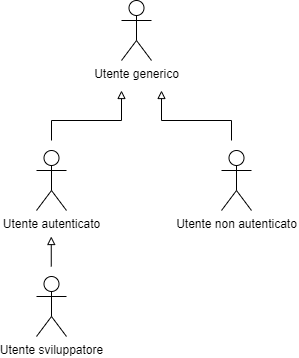
\includegraphics[scale=0.5]{./res/img/gerarchia.png}
			\caption {Gerarchia degli attori}
		\end{figure}
		\begin{description}[style=nextline]
			\item[\textbf{Utente generico}]
				Si riferisce ad un utente generico che ha avviato l'applicativo. 
			\item[\textbf{Utente non autenticato}]
				Si riferisce ad un utente generico che non ha ancora effettuato l'autenticazione all'interno della rete Ethereum\ped{\textit{G}}. 
			\item[\textbf{Utente autenticato}]
				Si riferisce ad un utente generico che si è autenticato nel sistema tramite il comando di login. Ciò implica che sia in possesso di una private key\ped{\textit{G}} o una mnemonic phrase\ped{\textit{G}} valida all'interno della rete Ethereum\ped{\textit{G}}. 
			\item[\textbf{Utente sviuppatore}] 
				Si riferisce ad un utente autenticato che ha svolto il deploy\ped{\textit{G}} di almeno una sua funzione. 
		\end{description}
	
	\subsubsection{Attori secondari}
		\begin{description}[style=nextline]
			\item[\textbf{Ethereum network}]
				Piattaforma decentralizzata utilizzata per la gestione dell'autenticazione, dei pagamenti e della comunicazione tra i vari moduli della piattaforma \textit{Etherless}. 
		\end{description}
	\pagebreak

\subsection{Elenco dei casi d'uso}
In questa sezione vengono elencati tutti i casi d'uso\ped{\textit{G}} individuati. Ogni caso d'uso\ped{\textit{G}} rappresenta uno scenario per uno o più attori, ed è descritto tramite degli appositi diagrammi dei casi d'uso\ped{\textit{G}}. 

\subsubsection{UC1 - Visualizzazione guida introduttiva}
	\begin{itemize}
		\item \textbf{Attori primari:} \ug{};
		\item \textbf{Descrizione:} dopo aver eseguito il comando \init{} il sistema mostra una guida contenente una breve spiegazione riguardante i comandi di \login{} e \signup{}. Tale guida ha lo scopo di aiutare l'utente a procedere nell'utilizzo dell'applicativo; 
		\item \textbf{Scenario principale:} 
		\begin{itemize}
			\item l’utente inserisce il comando \init{};
			\item viene visualizzata la guida introduttiva.
		\end{itemize}
		\item \textbf{Precondizione:} l'applicativo viene avviato correttamente e il sistema è raggiungibile;
		\item \textbf{Postcondizione:} vengono fornite all'utente tutte le informazioni necessarie per procedere con l'utilizzo dell'applicativo. 
	\end{itemize}
\subsubsection{UC2 - Aiuto comandi}
	\begin{figure}[h]
		\centering
		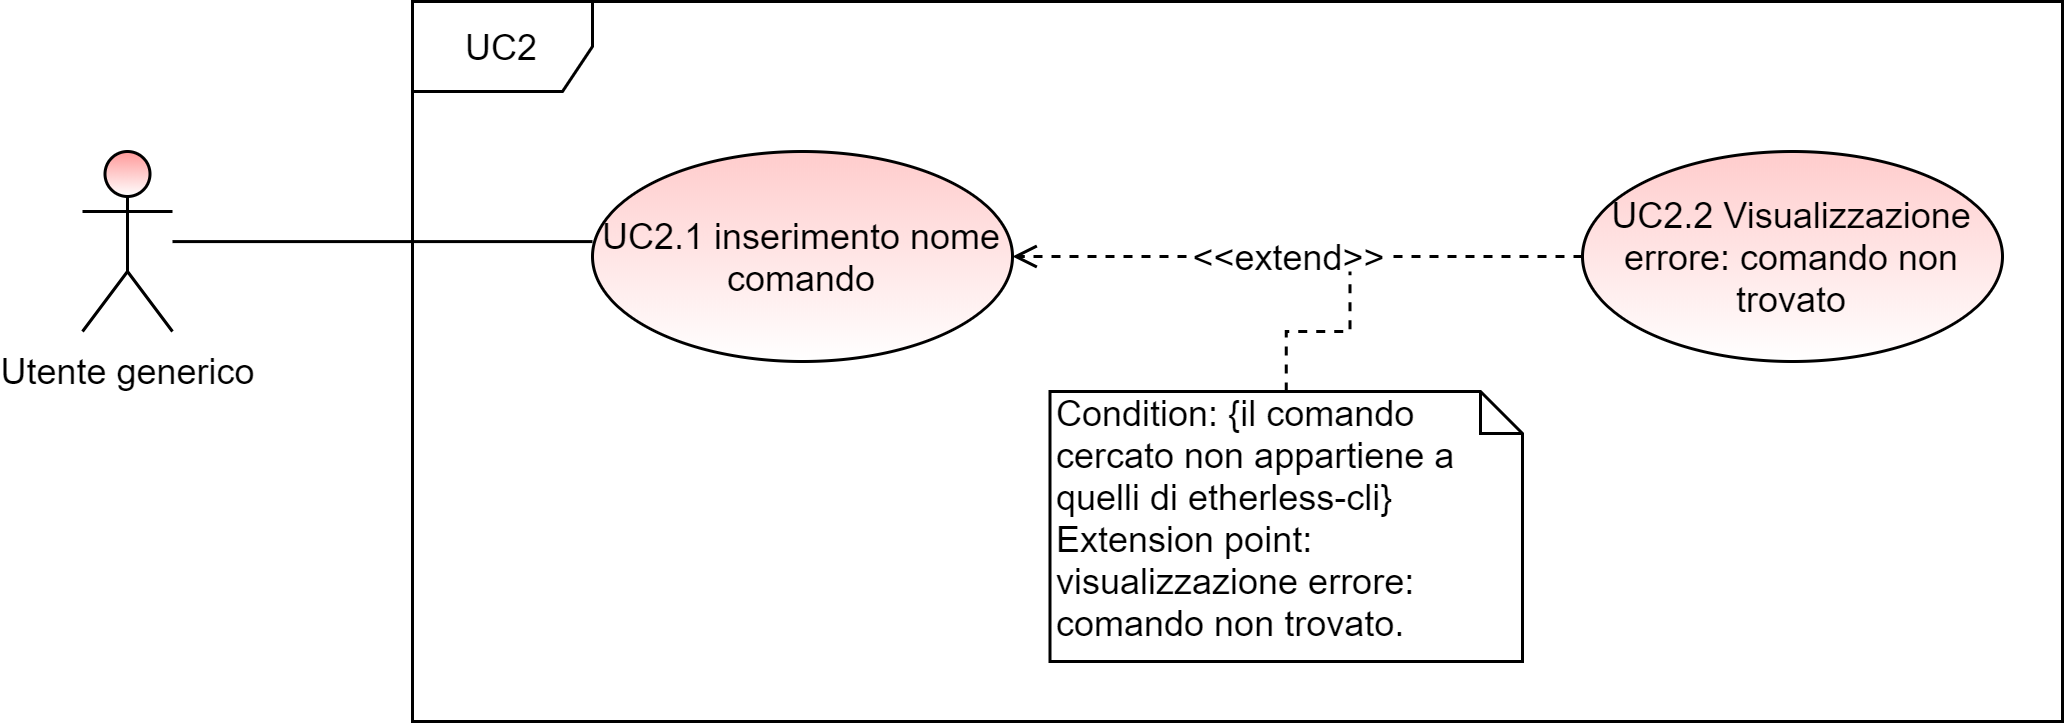
\includegraphics[scale=\ucs]{./res/img/UC2.png}
		\caption {UC2 - Aiuto comandi}
	\end{figure}
	\begin{itemize}
		\item \textbf{Attori primari:} \ug{};
		\item \textbf{Descrizione:} dopo aver inserito il comando \help{}, l’utente visualizza le informazioni dettagliate riguardo al comando desiderato;  
		\item \textbf{Scenario principale:} 
		\begin{itemize}
			\item l’utente inserisce il comando \phelp{};
			\item vengono visualizzate le informazioni dettagliate del comando richiesto. 
		\end{itemize}
		\item \textbf{Precondizione:} l’utente vuole ottenere maggiori informazioni riguardo ad un comando;
		\item \textbf{Postcondizione:} vengono visualizzate le informazioni dettagliate del comando di interesse.  
	\end{itemize}
\subsubsection{UC3 - Registrazione}
\begin{figure}[H]
	\centering
	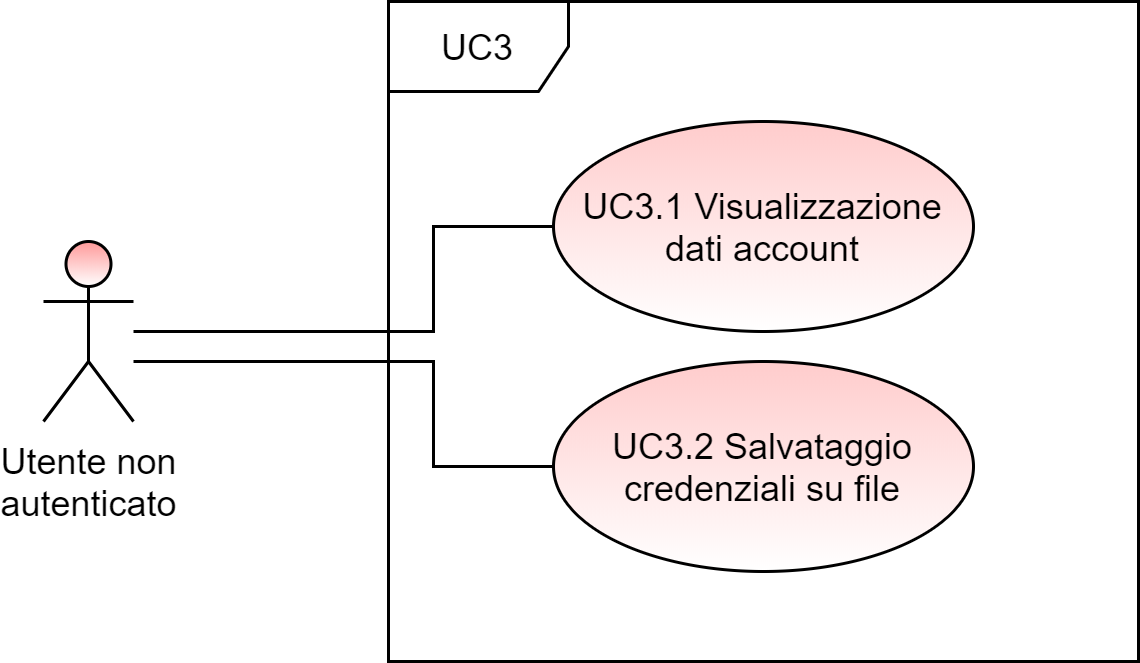
\includegraphics[scale=\ucs]{./res/img/UC3.png}
	\caption {UC3 - Registrazione}
\end{figure}
\begin{itemize}
	\item \textbf{Attori primari:} \una{};
	\item \textbf{Attori secondari:} \re{};
	\item \textbf{Descrizione:} dopo aver richiesto la creazione di un nuovo account Ethereum\ped{\textit{G}} tramite l’utilizzo del comando \signup{}, l’utente visualizza a video le credenziali del nuovo account creato; tali credenziali includono:
	\begin{itemize}
		\item address: indirizzo del nuovo account creato;
		\item private key\ped{\textit{G}}: chiave privata utilizzata per accedere alla rete Ethereum;
		\item mnemonic phrase\ped{\textit{G}}: frase composta da 12 parole, utilizzata per generare la chiave privata o per eseguire il login.
	\end{itemize}
	\item \textbf{Scenario principale:}
	\begin{itemize}
		\item l’utente richiede la creazione di un account all’interno della rete Ethereum\ped{\textit{G}} mediante il comando \signup{};
		\item vengono visualizzate le credenziali del nuovo account creato. 
	\end{itemize}
	\item \textbf{Precondizione:} l'utente vuole creare un nuovo account; 
	\item \textbf{Postcondizione:} l’account è stato creato correttamente. 
\end{itemize}
\subsubsection{UC3.1 - Visualizzazione dati account}
\begin{itemize}
	\item \textbf{Attori primari:} \una{};
	\item \textbf{Descrizione:} dopo la creazione di un nuovo account all’interno della rete Ethereum\ped{\textit{G}} il sistema mostra nella CLI\ped{\textit{G}} le relative credenziali;
	\item \textbf{Scenario principale:} l’utente visualizza le credenziali relative al nuovo account creato;  
	\item \textbf{Precondizione:} è stato creato correttamente un nuovo account nella rete Ethereum\ped{\textit{G}};   
	\item \textbf{Postcondizione:}  vengono mostrate a video le credenziali del nuovo account.  
\end{itemize}
\subsubsection{UC3.2 - Salvataggio credenziali su file}
\begin{itemize}
	\item \textbf{Attori primari:} \una{};
	\item \textbf{Descrizione:} l’utente può richiedere il salvataggio su file delle credenziali del nuovo account creato.
	\item \textbf{Scenario principale:}
	\begin{itemize}
		\item l’utente richiede di salvare su file le informazioni del nuovo account creato eseguendo il comando \signup{} seguito dal flag \texttt{-s}; 
		\item il sistema si occupa del corretto salvataggio delle credenziali. 
	\end{itemize}
	\item \textbf{Precondizione:} l’utente richiede di salvare le informazioni relative al nuovo eseguendo il comando \signup{} seguito dal flag \texttt{-s};  
	\item \textbf{Postcondizione:} le credenziali sono state salvate con successo all’interno del file.
\end{itemize}
\subsubsection{UC4 - Salvataggio credenziali su file}
\begin{figure}[h]
	\centering
	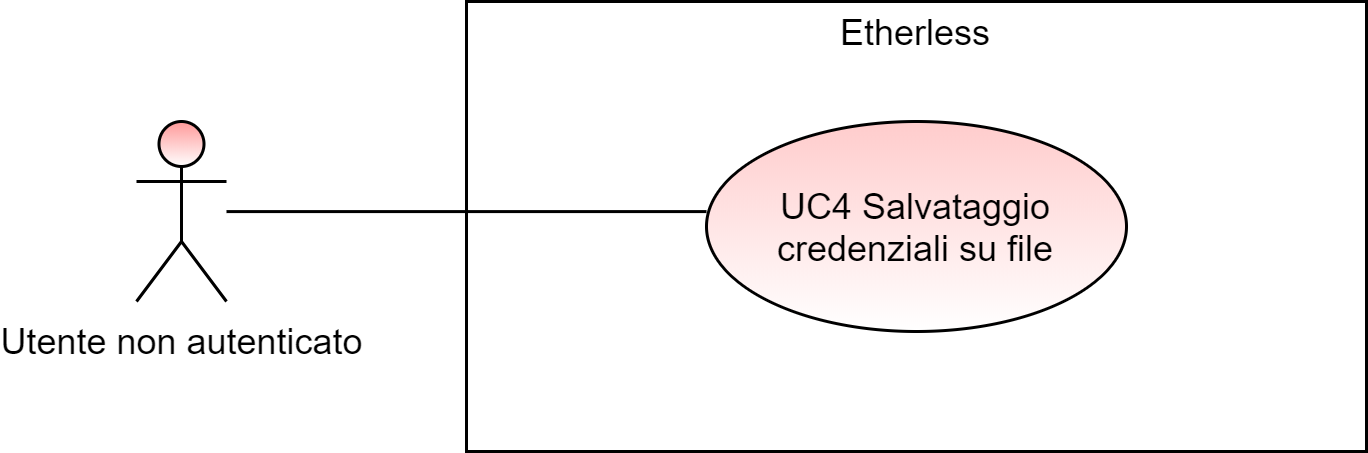
\includegraphics[scale=\ucs]{./res/img/UC4G.png}
	\caption {UC4 - Salvataggio credenziali su file: schema generale}
\end{figure}
\begin{itemize}
	\item \textbf{Attori primari:} \una{};
	\item \textbf{Descrizione:} a seguito della creazione di una nuova utenza Ethereum\ped{\textit{G}} l’utente può richiedere al sistema il salvataggio su file delle credenziali dell’account creato. Tali credenziali includono address, private key\ped{\textit{G}} e mnemonic phrase\ped{\textit{G}}.
	\item \textbf{Scenario principale:}
	\begin{itemize}
		\item l’utente richiede di salvare su file le informazioni del nuovo account creato; 
		\item il sistema si occupa del corretto salvataggio delle credenziali. 
	\end{itemize}
	\item \textbf{Precondizione:} l’utente richiede di salvare le informazioni relative al nuovo account tramite l’utilizzo del flag \texttt{-s};  
	\item \textbf{Postcondizione:} le credenziali sono state salvate con successo all’interno del file.  
\end{itemize}
\subsubsection{UC4.1 - Inserimento password}
\begin{itemize}
	\item \textbf{Attori primari:} \una{};
	\item \textbf{Descrizione:} al fine di terminare la procedura di autenticazione l’utente deve inserire una password per cifrare il proprio wallet\ped{\textit{G}};
	\item \textbf{Scenario principale:} l’utente procede con l’inserimento di 
	una password necessaria alla memorizzazione sicura del proprio wallet;  
	\item \textbf{Precondizione:} l’utente ha deciso di autenticarsi e ha già inserito
	il comando \texttt{login} seguito da private key\ped{\textit{G}} o mnemonic phrase\ped{\textit{G}} nella CLI\ped{\textit{G}}  
	\item \textbf{Postcondizione:} l’utente ha inserito correttamente una password. 
\end{itemize}
\subsubsection{UC5 - Login con private key}
\begin{figure}[H]
	\centering
	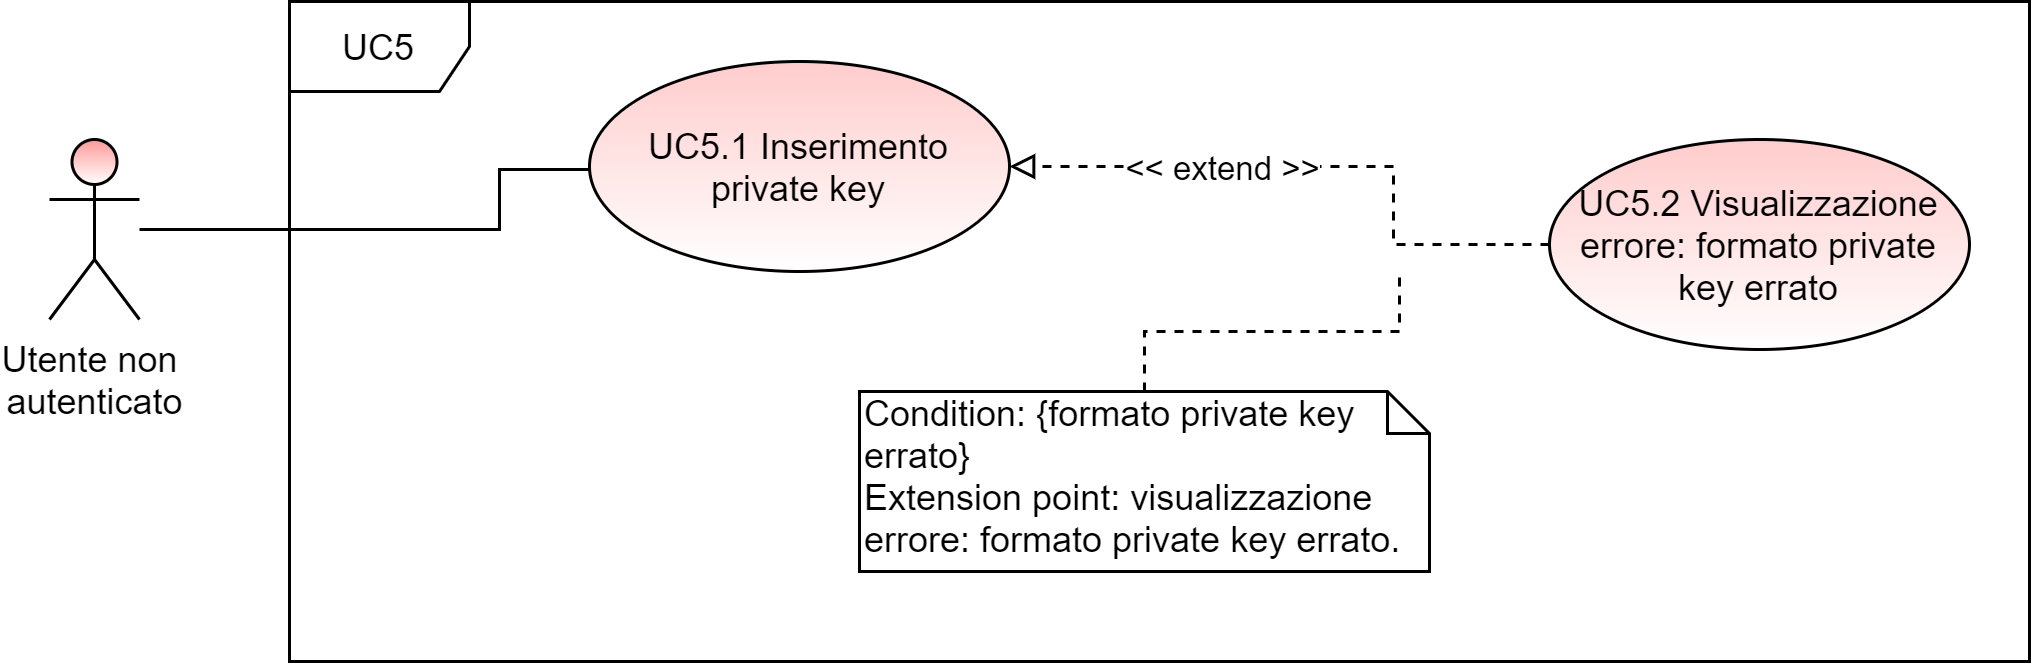
\includegraphics[scale=\ucs]{./res/img/UC5.png}
	\caption {UC5 - Login con private key}
\end{figure}
\begin{itemize}
	\item \textbf{Attori primari:} \una{};
	\item \textbf{Attori secondari:} \re{};
	\item \textbf{Descrizione:} l’utente può utilizzare il comando \ploginPrivate{} per autenticarsi all’interno della rete Ethereum\ped{\textit{G}}; 
	\item \textbf{Scenario principale:} l'utente esegue il comando \login{} indicando manualmente le credenziali necessarie; 
	\item \textbf{Precondizione:} l’utente tenta di autenticarsi alla piattaforma;
	\item \textbf{Postcondizione:} l’utente si è autenticato correttamente.
\end{itemize}

\subsubsection{UC5.1 - Inserimento credenziali di accesso }
\begin{figure}[h]
	\centering
	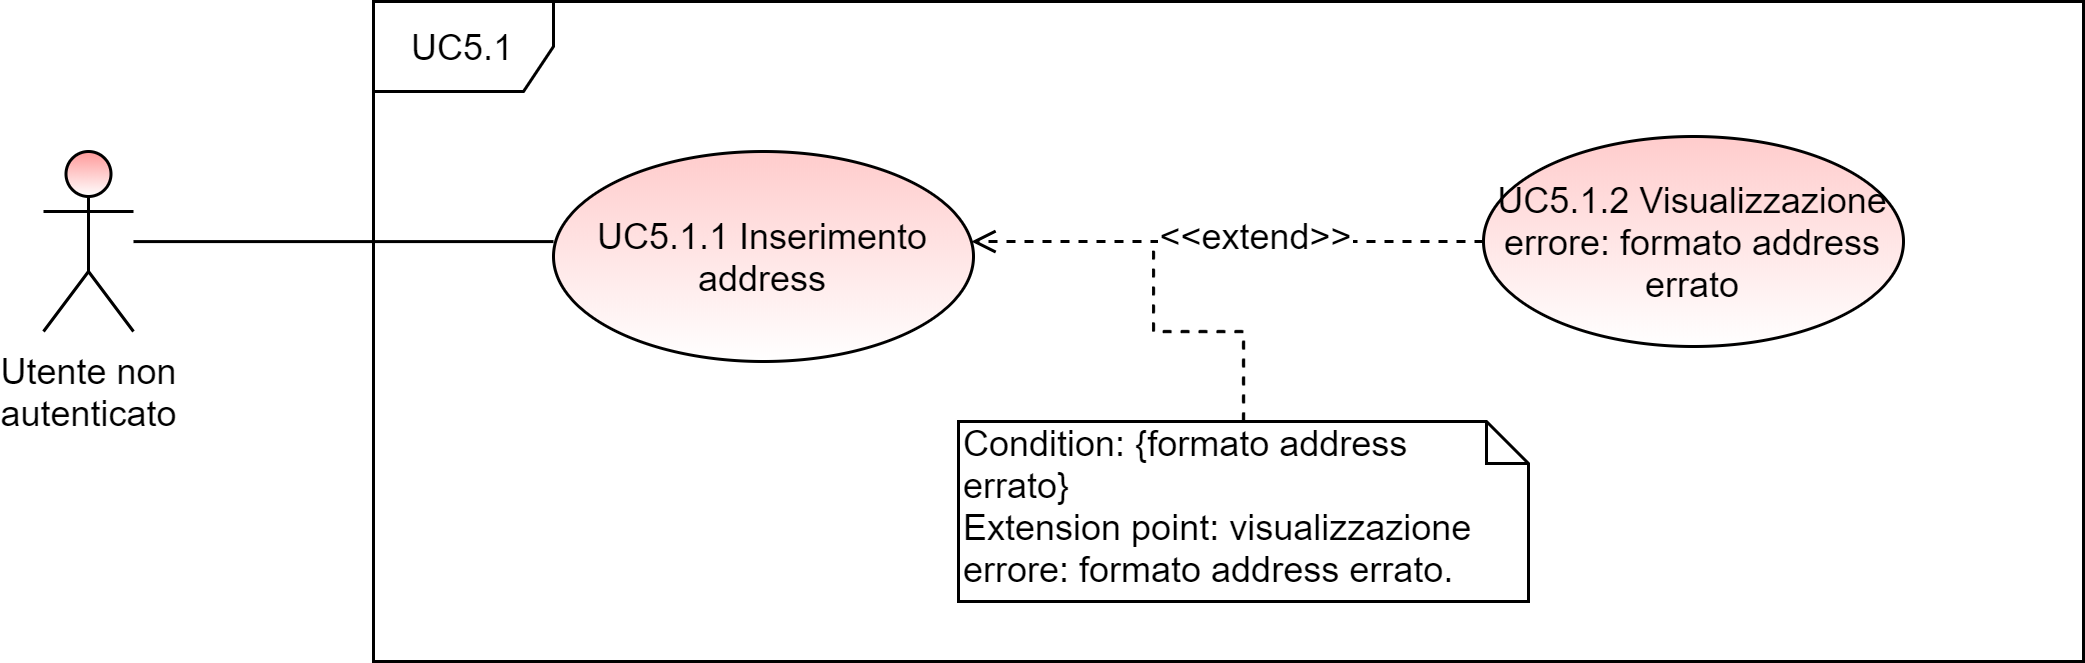
\includegraphics[scale=\ucs]{./res/img/UC5.1.png}
	\caption {UC5.1 - Inserimento credenziali di accesso }
\end{figure}
\begin{itemize}
	\item \textbf{Attori primari:} \una{};
	\item \textbf{Attori secondari:} \re{};
	\item \textbf{Descrizione:} l’utente procede all’inserimento delle credenziali necessarie per l'autenticazione. Oltre all’inserimento obbligatorio dell’address viene richiesta, a scelta dell’utente, la private key\ped{\textit{G}} o mnemonic phrase\ped{\textit{G}}; 
	\item \textbf{Scenario principale:} l'utente provvede ad inserire le credenziali necessarie per l’accesso.  
	\item \textbf{Specializzazioni:} 
	\begin{itemize}
		\item \textbf{UC5.2:} l’utente decide di eseguire il login tramite private key\ped{\textit{G}};
		\item \textbf{UC5.3:} ’utente decide di eseguire il login tramite mnemonic phrase\ped{\textit{G}}.
	\end{itemize}
	\item \textbf{Estensioni:} 
	\begin{itemize}
		\item \textbf{UC5.6:} se le credenziali inserite sono errate allora il sistema mostra un messaggio di errore.  
	\end{itemize}
	\item \textbf{Precondizione:}  l’utente ha inserito il comando \login{};   
	\item \textbf{Postcondizione:} l'utente ha inserito correttamente le credenziali per effettuare l’accesso. 
\end{itemize}
\subsubsection{UC5.2 - Inserimento private key }
\begin{itemize}
	\item \textbf{Attori primari:} \una{};
	\item \textbf{Descrizione:} al fine di terminare la procedura di autenticazione l’utente deve inserire la propria private key;
	\item \textbf{Scenario principale:} dopo aver deciso di volersi autenticare tramite l’utilizzo della propria private key, l’utente procede con l’inserimento di quest’ultima;  
	\item \textbf{Estensioni:} 
	\begin{itemize}
		\item \textbf{UC5.4:} nel caso di inserimento di una private key in formato errato viene mostrato un messaggio di errore.
	\end{itemize}
	\item \textbf{Precondizione:} l’utente ha deciso di autenticarsi tramite uso della propria private key e ha già inserito nella CLI il comando login seguito dal suo address; 
	\item \textbf{Postcondizione:} l’utente ha inserito correttamente la propria private key. 
\end{itemize}
\subsubsection{UC6 - Login con mnemonic phrase}
\begin{figure}[h]
	\centering
	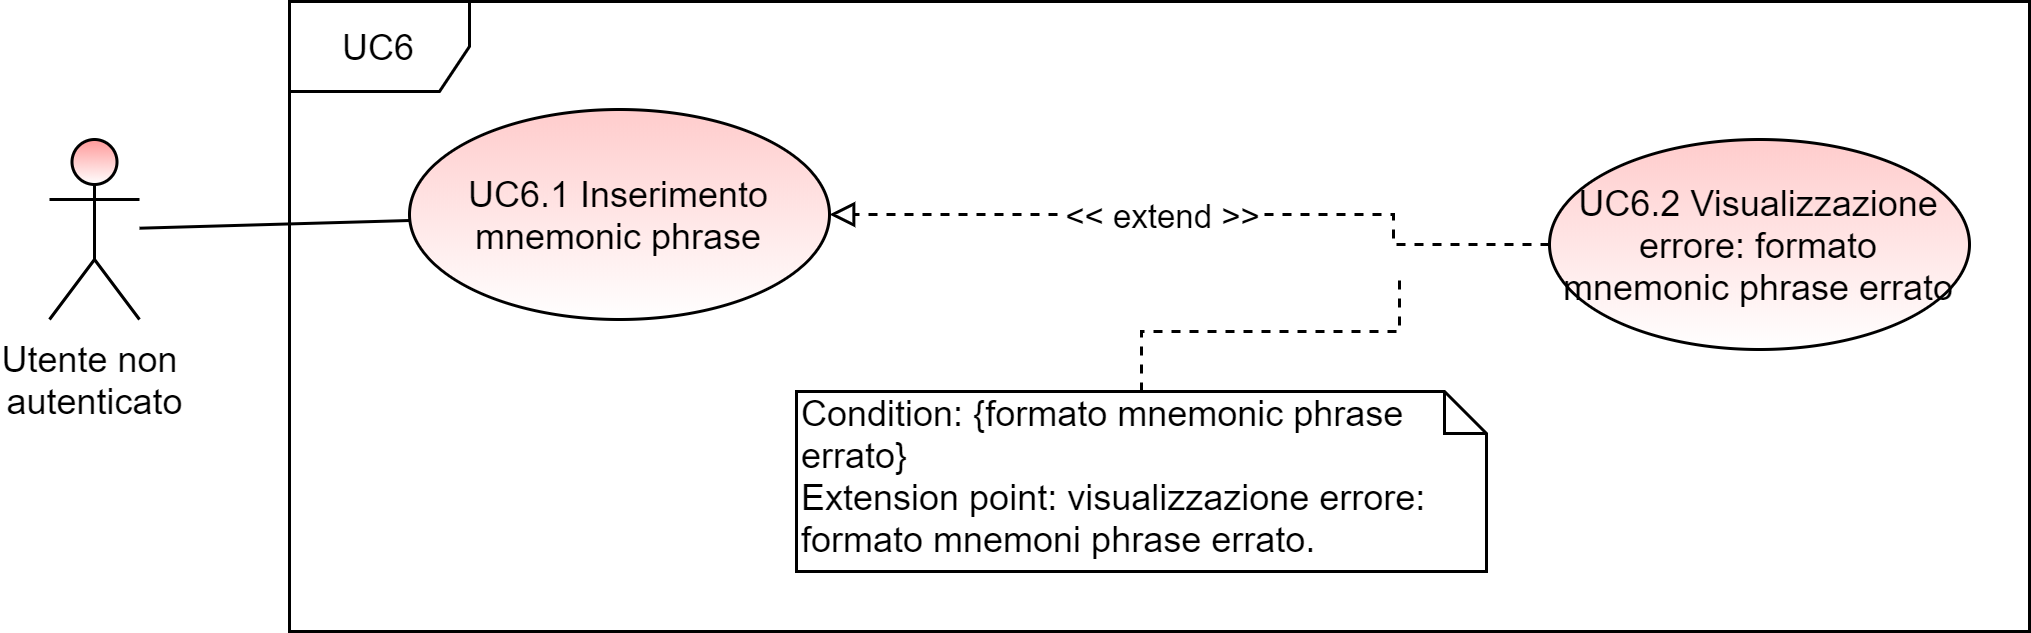
\includegraphics[scale=\ucs]{./res/img/UC6.png}
	\caption {UC6 - Login con mnemonic phrase\ped{\textit{G}}}
\end{figure}
\begin{itemize}
	\item \textbf{Attori primari:} \una{};
	\item \textbf{Attori secondari:} \re{};
	\item \textbf{Descrizione:} l’utente può utilizzare il comando \ploginMnemonic{} per autenticarsi all’interno della rete Ethereum\ped{\textit{G}}; 
	\item \textbf{Scenario principale:} l'utente esegue il comando \login{} indicando manualmente le credenziali necessarie; 
	\item \textbf{Precondizione:} l’utente tenta di autenticarsi alla piattaforma;
	\item \textbf{Postcondizione:} l’utente si è autenticato correttamente.
\end{itemize}
\subsubsection{UC6.1 - Inserimento private key }
\begin{itemize}
	\item \textbf{Attori primari:} \una{};
	\item \textbf{Descrizione:} al fine di terminare la procedura di autenticazione l’utente deve inserire la propria private key\ped{\textit{G}};
	\item \textbf{Scenario principale:} dopo aver deciso di volersi autenticare tramite l’utilizzo della propria private key\ped{\textit{G}}, l’utente procede con l’inserimento di quest’ultima;  
	\item \textbf{Estensioni:} 
	\begin{itemize}
		\item \textbf{UC6.3:} nel caso di inserimento di una private key\ped{\textit{G}} in formato errato viene mostrato un messaggio di errore.
	\end{itemize}
	\item \textbf{Precondizione:} l’utente ha deciso di autenticarsi tramite uso della propria private key\ped{\textit{G}} e ha già inserito nella CLI\ped{\textit{G}} il comando \texttt{login}; 
	\item \textbf{Postcondizione:} l’utente ha inserito correttamente la propria private key\ped{\textit{G}}. 
\end{itemize}
\subsubsection{UC6.2 - Inserimento password}
\begin{itemize}
	\item \textbf{Attori primari:} \una{};
	\item \textbf{Descrizione:} al fine di terminare la procedura di autenticazione l’utente deve inserire una password per cifrare il proprio wallet\ped{\textit{G}};
	\item \textbf{Scenario principale:} l’utente procede con l’inserimento di 
	una password necessaria alla memorizzazione sicura del proprio wallet;  
	\item \textbf{Precondizione:} l’utente ha deciso di autenticarsi tramite uso della propria private key\ped{\textit{G}} e ha già inserito nella CLI\ped{\textit{G}} il comando \texttt{login} seguito dalla private key\ped{\textit{G}}; 
	\item \textbf{Postcondizione:} l’utente ha inserito correttamente una password. 
\end{itemize}
\subsubsection{UC7 - Login automatico}
\begin{figure}[H]
	\centering
	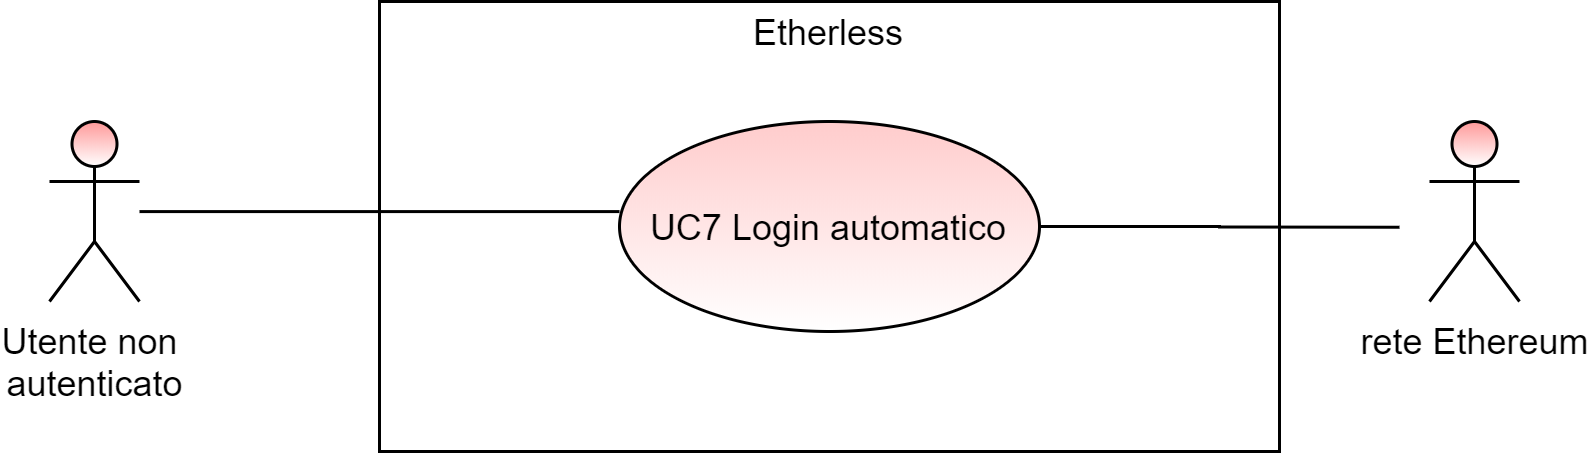
\includegraphics[scale=\ucs]{./res/img/UC7G.png}
	\caption {UC7 - Login automatico: schema generale}
\end{figure}
\begin{itemize}
	\item \textbf{Attori primari:} \una{};
	\item \textbf{Attori secondari:} \re{};
	\item \textbf{Descrizione:} in maniera automatica il sistema si occupa dell’autenticazione dell’utente;
	\item \textbf{Scenario principale:} l’utente avvia l'applicativo tramite il comando \init{} e viene autenticato in maniera automatica; 
	\item \textbf{Precondizione:} l’utente ha eseguito il login manuale almeno una volta, indicando esplicitamente la volontà di essere ricordato [\textbf{UC6}];
	\item \textbf{Postcondizione:} l’utente si è autenticato con successo
\end{itemize}
\subsubsection{UC8 - Disconnessione dal servizio}
\begin{figure}[h]
	\centering
	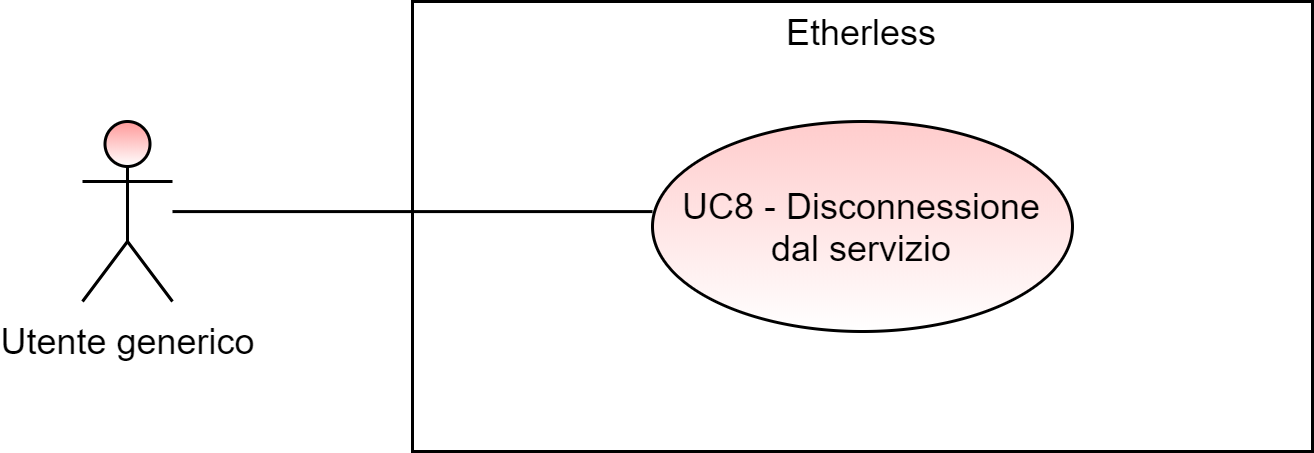
\includegraphics[scale=\ucs]{./res/img/UC8G.png}
	\caption {UC8 - Disconnessione dal servizio: schema generale}
\end{figure}
\begin{itemize}
	\item \textbf{Attori primari:} \ua{};
	\item \textbf{Descrizione:} l’utente richiede la disconnessione dal servizio eseguendo il comando \logout{}. Il sistema effettua la disconnessione; 
	\item \textbf{Scenario principale:} 
	\begin{itemize}
		\item l'utente inserisce correttamente ed esegue il comando \logout{}; 
		\item l'utente viene disconnesso dal servizio. 
	\end{itemize}
	\item \textbf{Precondizione:} l’utente è stato autenticato correttamente e richiede di essere disconnesso; 
	\item \textbf{Postcondizione:} l’utente viene disconnesso con successo..
\end{itemize}

\subsubsection{UC9 - Visualizzazione address utente}
\begin{figure}[h]
	\centering
	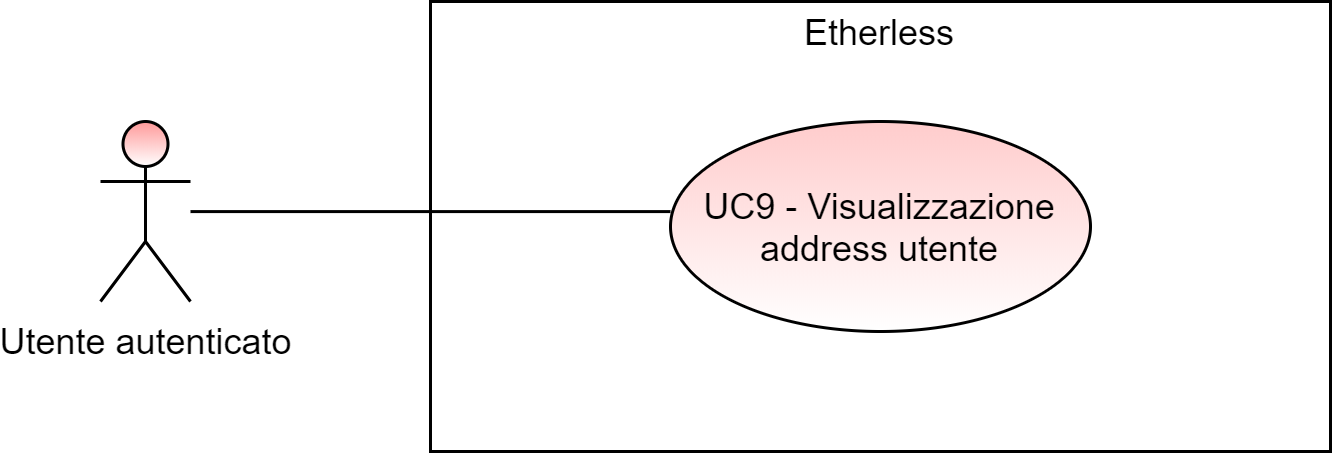
\includegraphics[scale=\ucs]{./res/img/UC9G.png}
	\caption {UC9 - Visualizzazione address utente: schema generale}
\end{figure}
\begin{itemize}
	\item \textbf{Attori primari:} \ua{};
	\item \textbf{Descrizione:} l’utente richiede la visualizzazione del campo address associato al proprio account eseguendo il comando \whoami{}. Il sistema stampa a video tale informazione; 
	\item \textbf{Scenario principale:} 
	\begin{itemize}
		\item l'utente inserisce correttamente ed esegue il comando \whoami{}; 
		\item il sistema visualizza il campo address associato all’utente
	\end{itemize}  
	\item \textbf{Precondizione:} l’utente è stato autenticato correttamente e richiede di visualizzare l’indirizzo associato alla propria utenza;
	\item \textbf{Postcondizione:} la CLI riporta il campo address associato all’account dell’utente.
\end{itemize}
\subsubsection{UC9.1 - Inserimento nome funzione}
\begin{itemize}
	\item \textbf{Attori primari:} \ua{};
	\item \textbf{Descrizione:} l’utente inserisce il nome della funzione della quale desidera visualizzare la descrizione completa;
	\item \textbf{Scenario principale:} l'utente inserisce il comando \info{} seguito dal nome della funzione;
	\item \textbf{Estensioni:} 
	\begin{itemize}
		\item \textbf{UC9.3:} l’utente inserisce un nome non presente nel sistema, viene quindi visualizzato un messaggio di errore.
	\end{itemize}
	\item \textbf{Precondizione:} l'utente ha digitato il comando \info{};
	\item \textbf{Postcondizione:} l’utente ha inserito correttamente il nome della funzione.
\end{itemize}

\subsubsection{UC10 - Ricerca funzione per nome}
\begin{figure}[H]
	\centering
	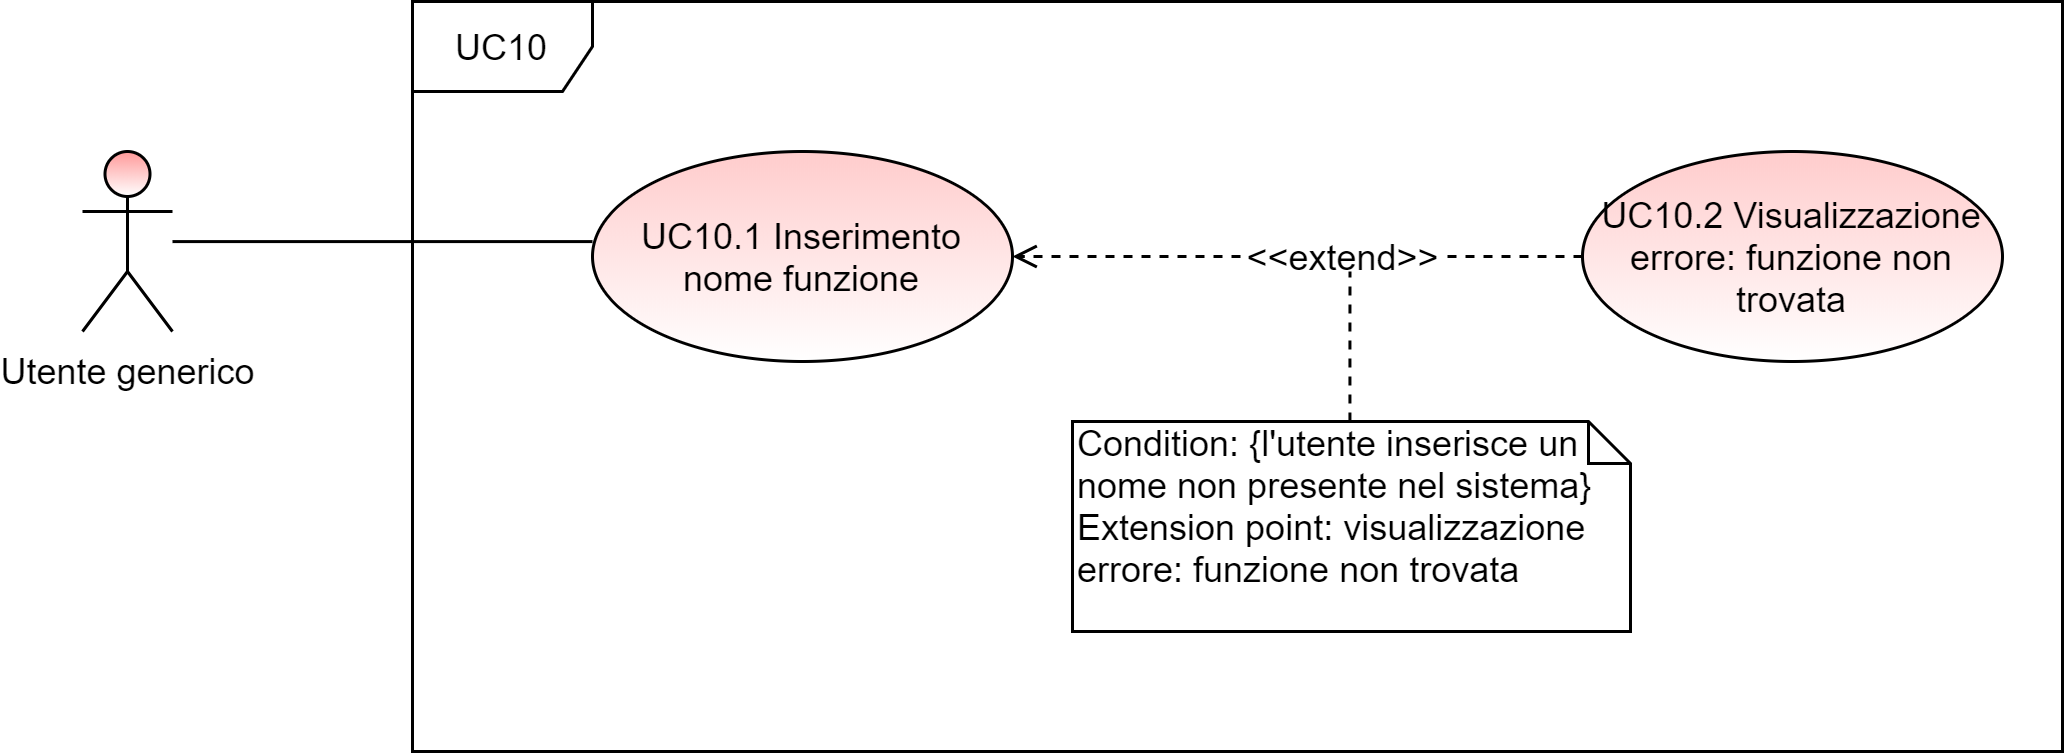
\includegraphics[scale=\ucs]{./res/img/UC10.png}
	\caption {UC10 - Ricerca funzione per nome}
\end{figure}
\begin{itemize}
	\item \textbf{Attori primari:} \ua{};
	\item \textbf{Attori secondari:} \re{};
	\item \textbf{Descrizione:} l’utente richiede di eseguire la ricerca di tutte le funzioni il cui nome contiene un certo termine di ricerca eseguendo il comando \psearch{}.
	\item \textbf{Scenario principale:} 
	\begin{itemize}
		\item l’utente inserisce correttamente ed esegue il comando \psearch{};
	\end{itemize}
	\item \textbf{Precondizione:} l’utente desidera individuare tutte le funzioni correlate ad un certo termine;
	\item \textbf{Postcondizione:} viene eseguita la ricerca di tutte le funzioni il cui nome contiene il termine di ricerca specificato nel comando \search{}.
\end{itemize}
\subsubsection{UC10.1 - Inserimento nome funzione}
\begin{itemize}
	\item \textbf{Attori primari:} \ua{};
	\item \textbf{Descrizione:} l’utente inserisce il nome della funzione della quale desidera visualizzare le informazioni generali;
	\item \textbf{Scenario principale:} l'utente inserisce il comando \info{} seguito dal nome della funzione;
	\item \textbf{Estensioni:} 
	\begin{itemize}
		\item \textbf{UC10.2:} l’utente inserisce un nome non presente nel sistema, viene quindi visualizzato un messaggio di errore.
	\end{itemize}
	\item \textbf{Precondizione:} l'utente ha digitato il comando \info{};
	\item \textbf{Postcondizione:} l’utente ha inserito correttamente il nome della funzione.
\end{itemize}

\subsubsection{UC11 - Visualizzazione risultati ricerca tramite keyword}
\begin{figure}[H]
	\centering
	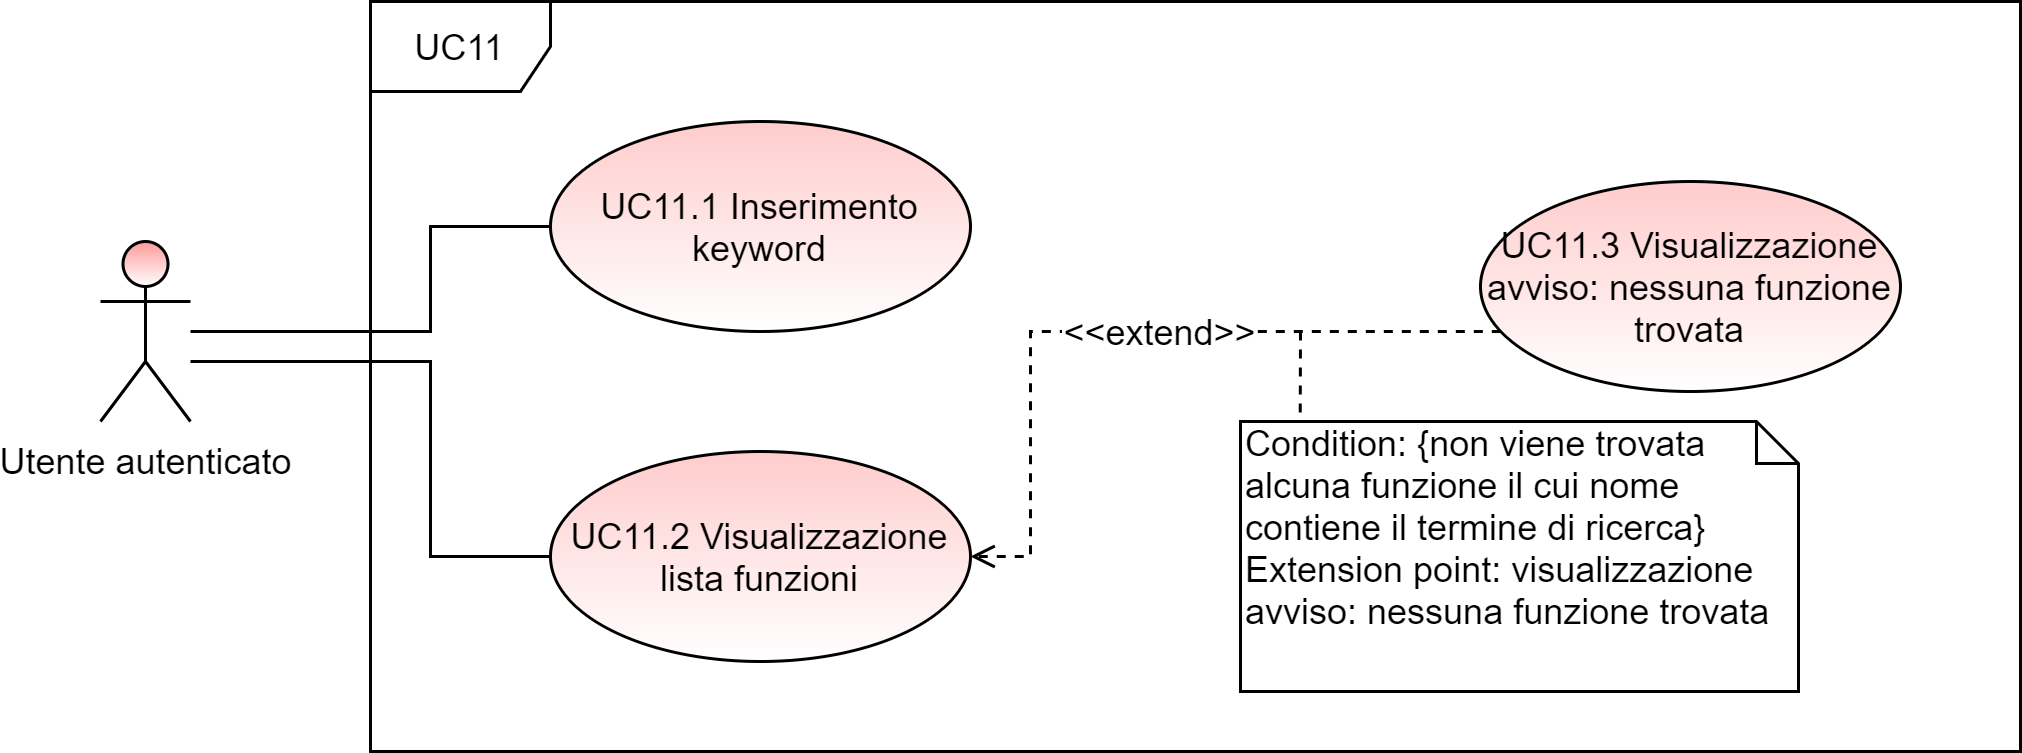
\includegraphics[scale=\ucs]{./res/img/UC11.png}
	\caption {UC11 - Visualizzazione risultati ricerca tramite keyword}
\end{figure}
\begin{itemize}
	\item \textbf{Attori primari:} \ua{};
	\item \textbf{Descrizione:} viene visualizzata la lista ritornata dal comando \texttt{search};
	\item \textbf{Scenario principale:} viene visualizzata una lista di tutte le funzioni che nel nome contengono il termine di ricerca specificato;
	\item \textbf{Estensioni:} 
	\begin{itemize}
		\item \textbf{UC12:} non viene trovata alcuna funzione il cui nome contiene il termine di ricerca. Viene di conseguenza visualizzato un messaggio di avviso.
	\end{itemize}
	\item \textbf{Precondizione:} l’utente ha inserito ed eseguito correttamente il comando \search{}, di conseguenza è stata eseguita la ricerca richiesta [UC10];
	\item \textbf{Postcondizione:} la CLI\ped{\textit{G}} riporta la lista di funzioni ritornata dal comando \search{}.
\end{itemize}
\subsubsection{UC11.1 - Inserimento keyword}
\begin{itemize}
	\item \textbf{Attori primari:} \ua{};
	\item \textbf{Descrizione:} l’utente inserisce, nel campo \textit{keyword}, il termine di ricerca che desidera individuare all’interno dei nomi delle funzioni disponibili nella piattaforma \textit{Etherless}; 
	\item \textbf{Scenario principale:} l'utente inserisce il termine di ricerca;
	\item \textbf{Precondizione:} l’utente ha digitato nella CLI il comando \search{};
	\item \textbf{Postcondizione:} l’utente inserisce correttamente il termine di ricerca. 
\end{itemize}

\subsubsection{UC12 - Visualizzazione avviso: nessuna funzione trovata}
\begin{itemize}
	\item \textbf{Attori primari:} \ua{};
	\item \textbf{Attori secondari:} \re{};
	\item \textbf{Descrizione:} l’utente richiede la visualizzazione della lista di tutte le funzioni il cui nome contiene un certo termine di ricerca eseguendo il comando \psearch{}. Nel sistema non è presente alcuna funzione che soddisfi tale criterio, di conseguenza viene visualizzato un messaggio di avviso;
	\item \textbf{Scenario principale:} viene visualizzato un messaggio di avviso relativo alla mancata presenza di funzioni il cui nome contiene il termine di ricerca specificato;
	\item \textbf{Precondizione:} l’utente ha inserito una keyword che non ha portato ad alcun risultato;
	\item \textbf{Postcondizione:} viene visualizzato un messaggio che descrive l'avviso.
\end{itemize}

\subsubsection{UC13 - Elenco funzioni}
\begin{figure}[H]
	\centering
	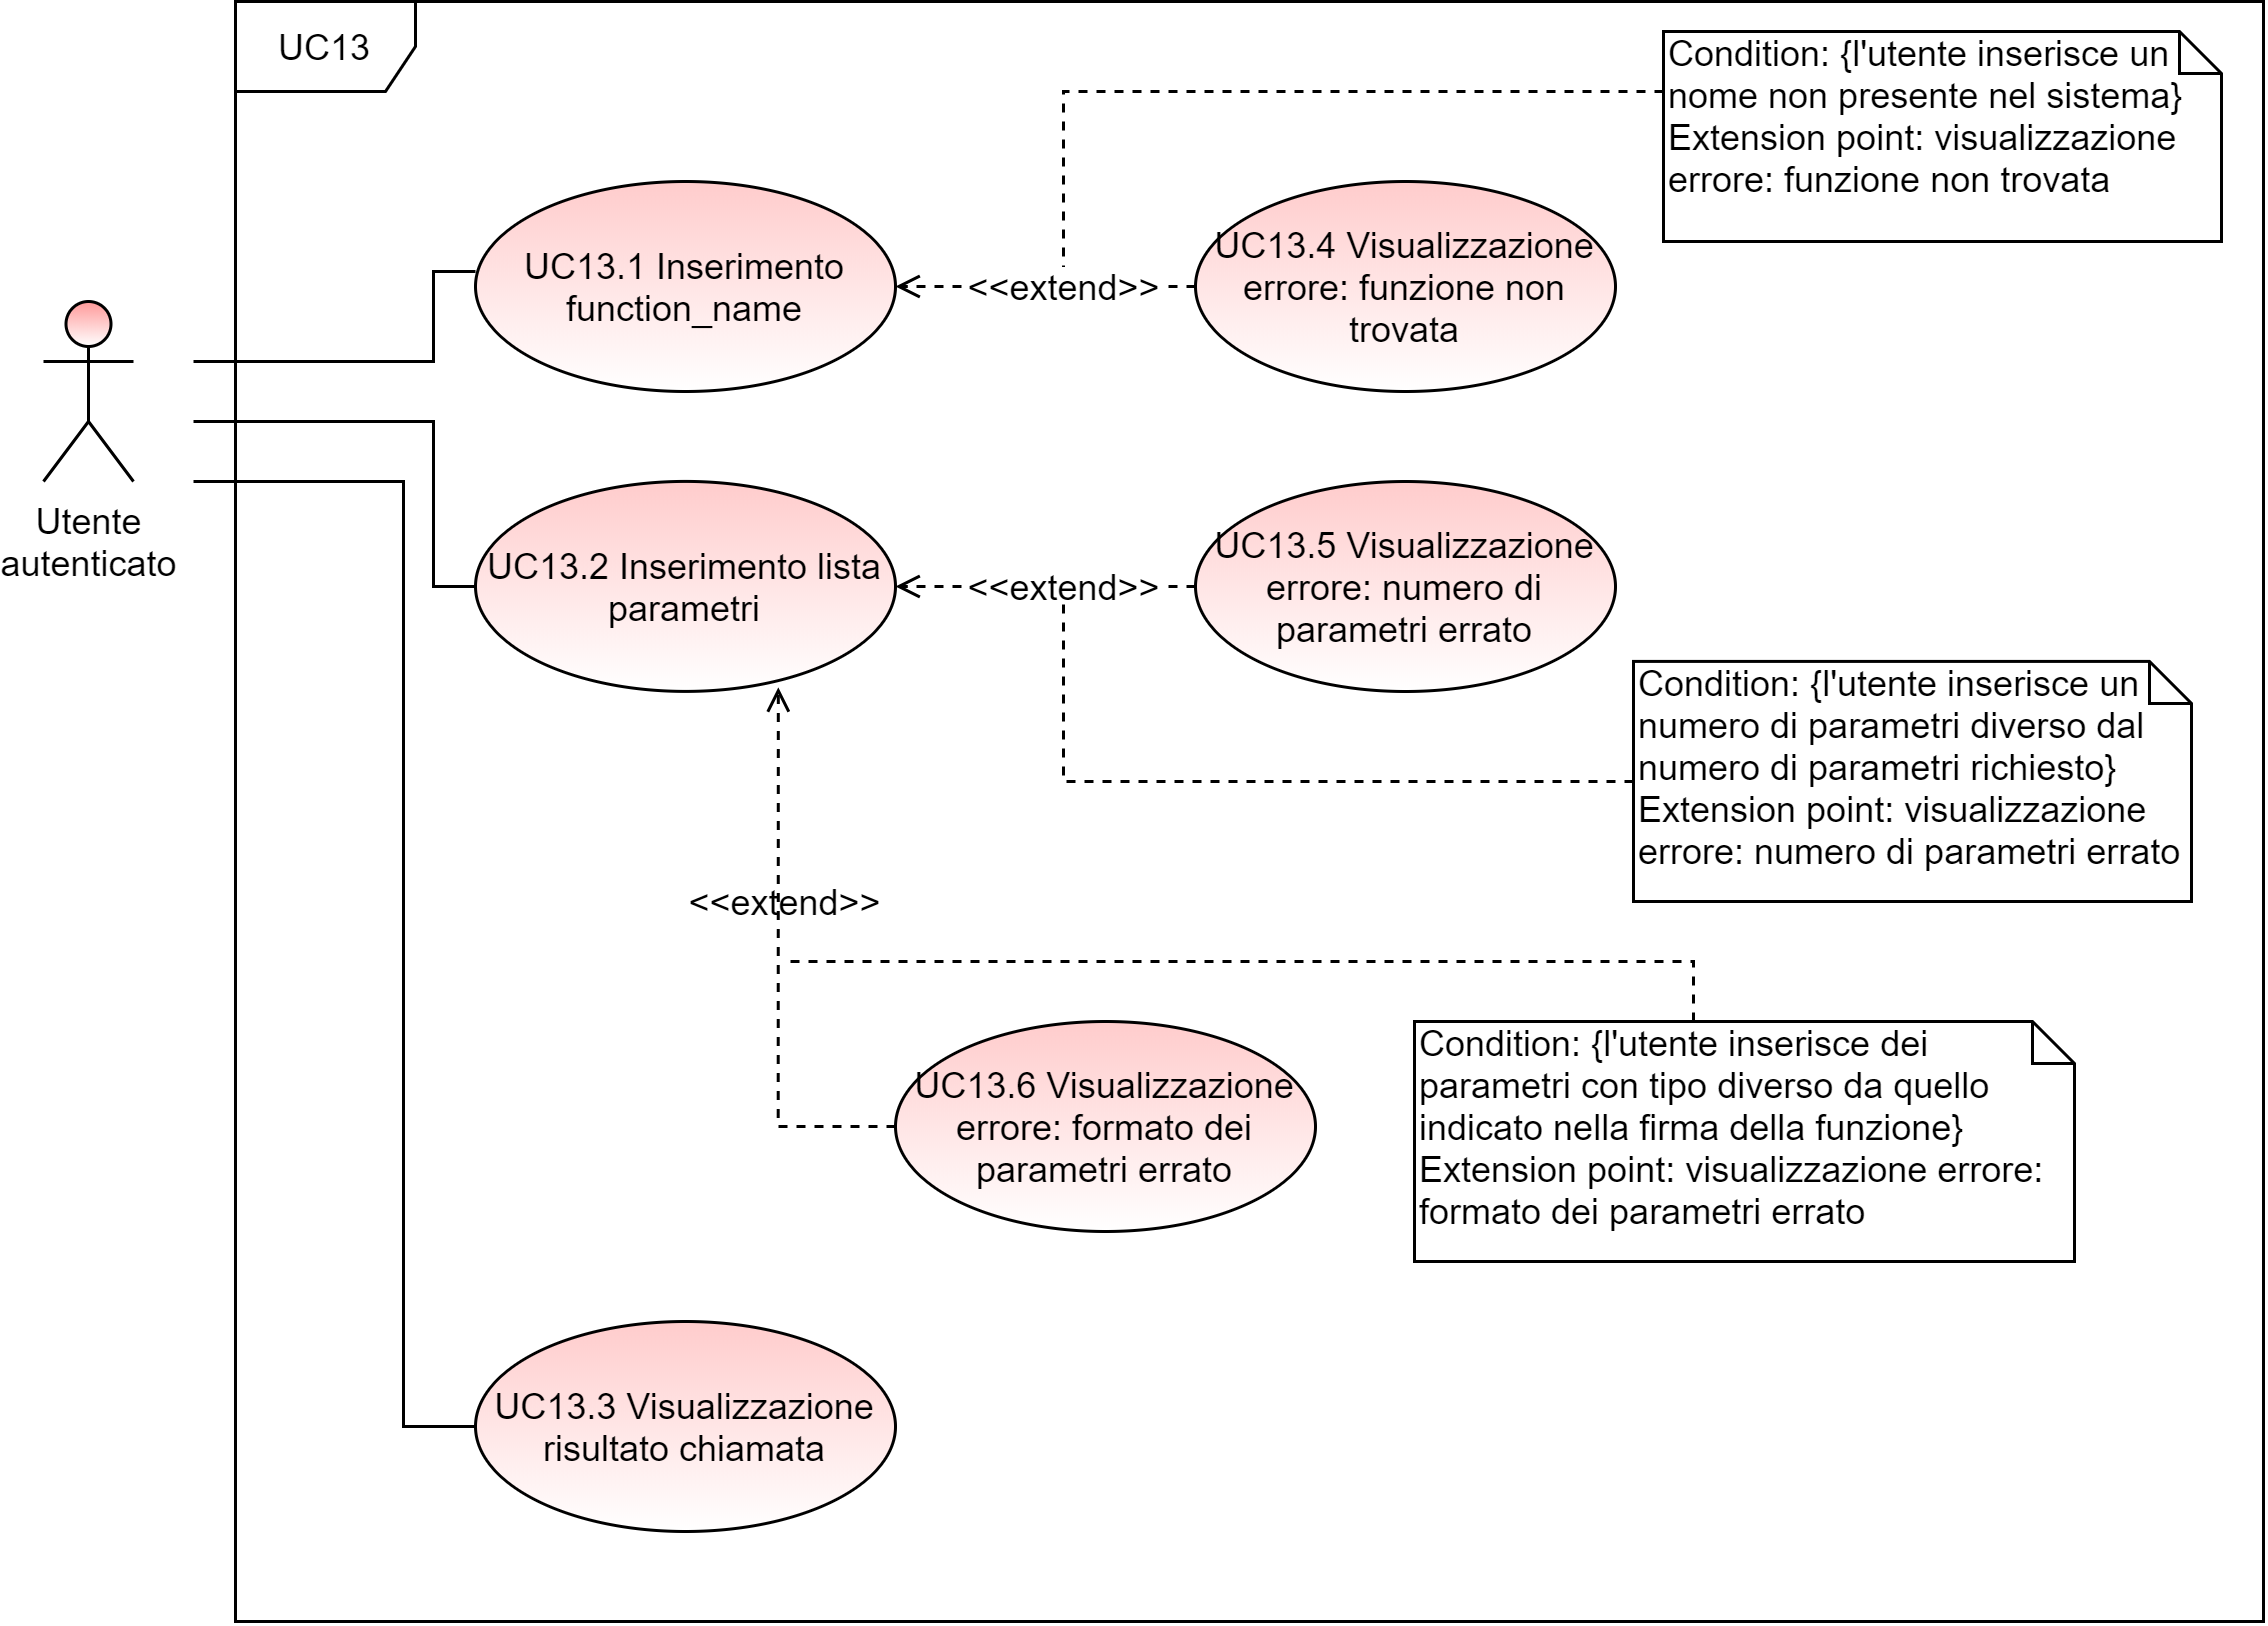
\includegraphics[scale=\ucs]{./res/img/UC13.png}
	\caption {UC13 - Elenco funzioni}
\end{figure}
\begin{itemize}
	\item \textbf{Attori primari:} \ua{};
	\item \textbf{Attori secondari:} \re{};
	\item \textbf{Descrizione:} l’utente richiede la visualizzazione della lista di tutte le funzioni disponibili presso il servizio oppure della lista delle funzioni di sua proprietà. Il sistema stampa a video tale lista.
	\item \textbf{Scenario principale:} 
	\begin{itemize}
		\item l'utente inserisce correttamente ed esegue il comando \lista{} oppure il comando \plista{}
		\item viene visualizzata la lista completa di tutte le funzioni disponibili oppure soltanto di quelle di proprietà dell’utente. 
	\end{itemize}
	\item \textbf{Precondizione:} l’utente desidera visualizzare la lista di tutte le funzioni oppure la lista delle funzioni di sua proprietà;
	\item \textbf{Postcondizione:} la CLI riporta la lista di tutte le funzioni disponibili oppure la lista delle funzioni di proprietà dell’utente.
\end{itemize}
\subsubsection{UC13.1 -  Visualizzazione lista di tutte le funzioni}
\begin{figure}[H]
	\centering
	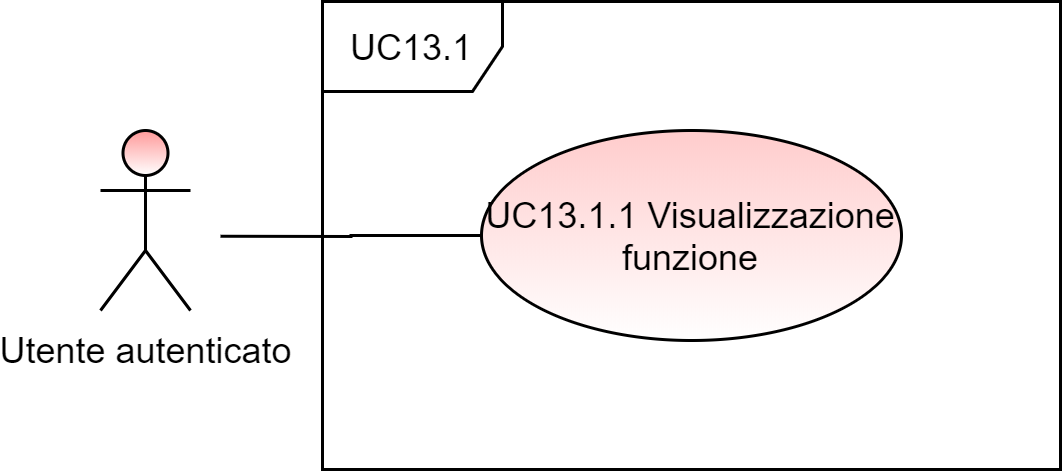
\includegraphics[scale=\ucs]{./res/img/UC13-1.png}
	\caption {UC13.1 -  Visualizzazione lista di tutte le funzioni}
\end{figure}
\begin{itemize}
	\item \textbf{Attori primari:} \ua{};
	\item \textbf{Descrizione:} l’utente richiede la visualizzazione della lista di tutte le funzioni fornite dal servizio eseguendo il comando list. Il sistema stampa a video tale lista; 
	\item \textbf{Scenario principale:} 
	\begin{itemize}
		\item l'utente inserisce correttamente ed esegue il comando \lista{}. 
		\item viene visualizzata la lista di tutte le funzioni disponibili presso il servizio;
	\end{itemize}
	\item \textbf{Estensioni:} 
	\begin{itemize}
		\item \textbf{UC13.3:} non è stata ancora pubblicata alcuna funzione, di conseguenza viene visualizzato un messaggio di avviso. 
	\end{itemize}
	\item \textbf{Precondizione:} l'utente inserisce correttamente ed esegue il comando \lista{};
	\item \textbf{Postcondizione:} la CLI\ped{\textit{G}} riporta la lista di tutte le funzioni fornite dal servizio.
\end{itemize}
\subsubsection{UC13.2 - Visualizzazione lista funzioni di proprietà dell’utente}
\begin{figure}[h]
	\centering
	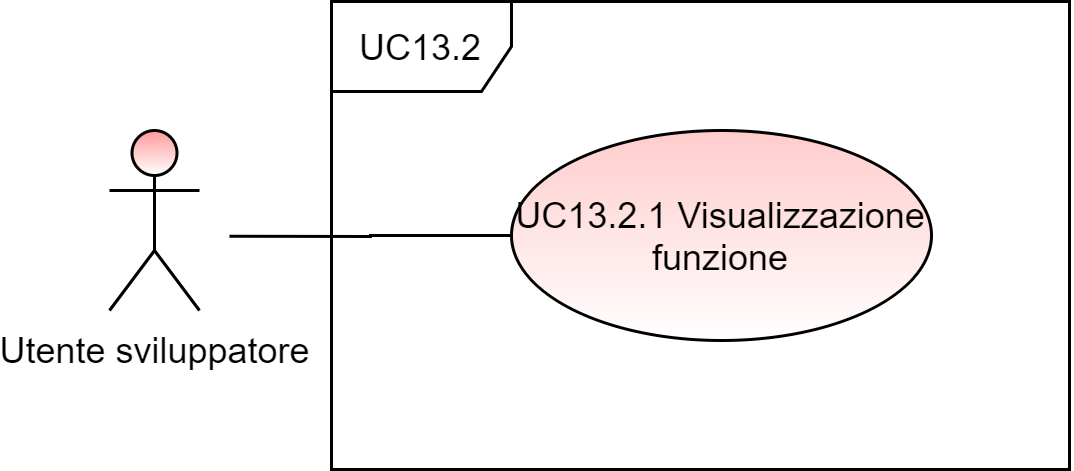
\includegraphics[scale=\ucs]{./res/img/UC13-2.png}
	\caption {UC13.2 - Visualizzazione lista funzioni di proprietà dell’utente}
\end{figure}
\begin{itemize}
	\item \textbf{Attori primari:} \us{};
	\item \textbf{Attori secondari:} \re{};
	\item \textbf{Descrizione:} l’utente richiede la visualizzazione della lista di tutte le funzioni di sua proprietà eseguendo il comando \plista{}. Il sistema stampa a video tale lista;
	\item \textbf{Scenario principale:} 
	\begin{itemize}
		\item l’utente inserisce correttamente ed esegue il comando \plista{};
		\item viene visualizzata la lista di tutte le funzioni di proprietà dell’utente. 
	\end{itemize}
	\item \textbf{Estensioni:} 
	\begin{itemize}
		\item \textbf{UC13.4:} l’utente non ha ancora pubblicato alcuna funzione, di conseguenza viene visualizzato un messaggio di avviso. 
	\end{itemize}
	\item \textbf{Precondizione:} l'utente inserisce correttamente ed esegue il comando \plista{};
	\item \textbf{Postcondizione:} la CLI\ped{\textit{G}} riporta la lista di tutte le funzioni di proprietà dell’utente. 
\end{itemize}
\subsubsection{UC13.3 - Visualizzazione risultato della chiamata}
\begin{itemize}
	\item \textbf{Attori primari:} \ua{};
	\item \textbf{Descrizione:} Viene visualizzato il risultato dell'esecuzione della funzione; 
	\item \textbf{Scenario principale:} viene visualizzato il risultato della chiamata;
	\item \textbf{Precondizione:} l’esecuzione della funzione è andata a buon fine; 
	\item \textbf{Postcondizione:} la CLI\ped{\textit{G}} riporta il risultato della chiamata.  
\end{itemize}
\subsubsection{UC13.4 - Visualizzazione errore: funzione non trovata}
\begin{itemize}
	\item \textbf{Attori primari:} \ua{};
	\item \textbf{Descrizione:}  l’utente richiede l’esecuzione di una funzione specificando un nome non presente nel sistema. Il sistema riporta un messaggio di errore relativo alla mancata presenza della funzione;
	\item \textbf{Scenario principale:} viene visualizzato un messaggio di errore relativo alla mancata presenza di una funzione con il nome specificato; 
	\item \textbf{Precondizione:} il nome inserito dall’utente non si riferisce ad alcuna funzione presente all’interno del sistema;  
	\item \textbf{Postcondizione:} viene visualizzato un messaggio che descrive l’errore considerato. 
\end{itemize}
\subsubsection{UC13.5 - Visualizzazione errore: numero di parametri errato}
\begin{itemize}
	\item \textbf{Attori primari:} \ua{};
	\item \textbf{Attori secondari:} \re{};
	\item \textbf{Descrizione:} l’utente richiede l’esecuzione di una funzione inserendo un numero di parametri diverso dal numero di parametri richiesto. Il sistema riporta un messaggio di errore relativo al numero errato di parametri;
	\item \textbf{Scenario principale:} viene visualizzato un messaggio di errore relativo al numero errato di parametri;
	\item \textbf{Precondizione:} il numero di parametri inseriti dall’utente non corrisponde a quelli indicati nella firma della funzione;
	\item \textbf{Postcondizione:} la CLI\ped{\textit{G}} riporta un messaggio di errore.
\end{itemize}
\subsubsection{UC13.6 - Visualizzazione errore: formato parametri errato}
\begin{itemize}
	\item \textbf{Attori primari:} \ua{};
	\item \textbf{Descrizione:} l’utente richiede l’esecuzione di una funzione inserendo dei parametri il cui tipo non coincide con quello indicato nella firma della funzione. Il sistema riporta un messaggio di errore relativo al formato dei parametri inseriti;
	\item \textbf{Scenario principale:} viene visualizzato un messaggio di errore relativo all'errato formato dei parametri;
	\item \textbf{Precondizione:} il  tipo dei parametri inseriti dall'utente non coincide con quello indicato nella firma della funzione; 
	\item \textbf{Postcondizione:} la CLI\ped{\textit{G}} riporta un messaggio di errore.
\end{itemize}

\subsubsection{UC14 - Deploy di funzione}
\begin{figure}[h]
	\centering
	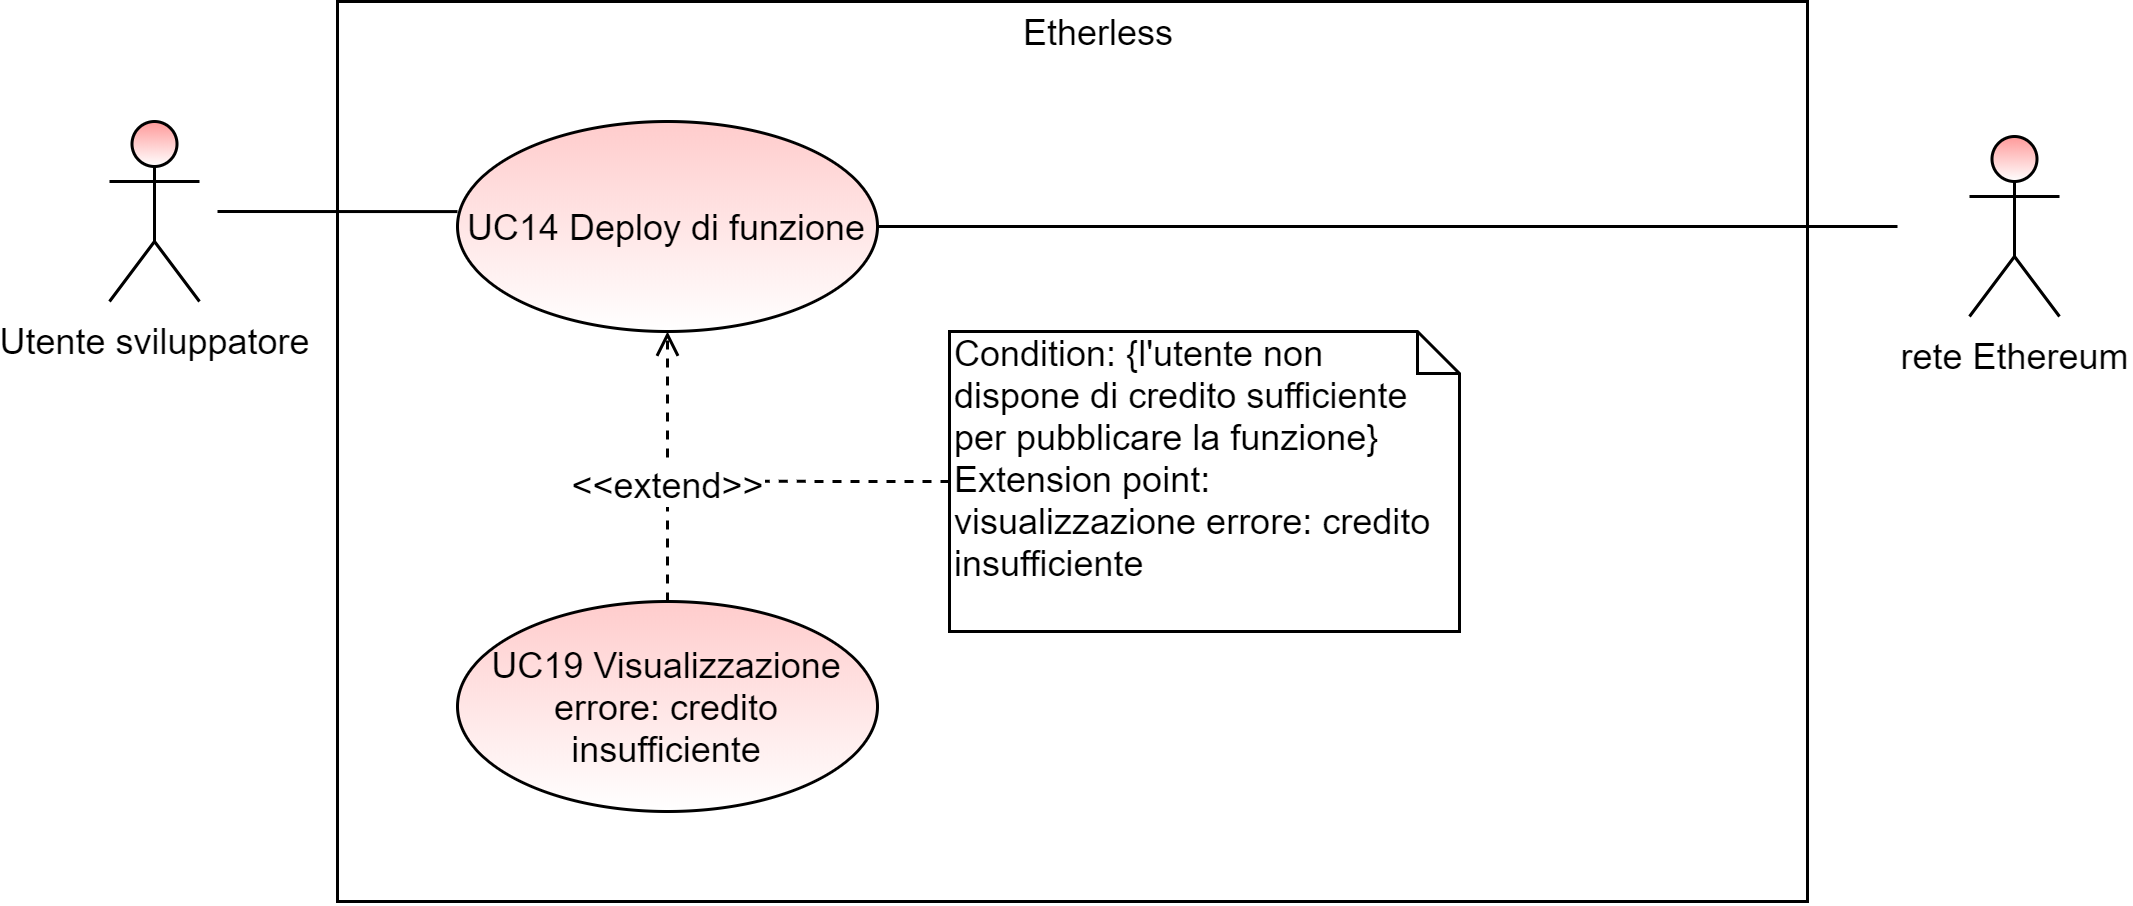
\includegraphics[scale=\ucs]{./res/img/UC14G.png}
	\caption {UC14 - Deploy di funzione: schema generale}
\end{figure}
\begin{figure}[h]
	\centering
	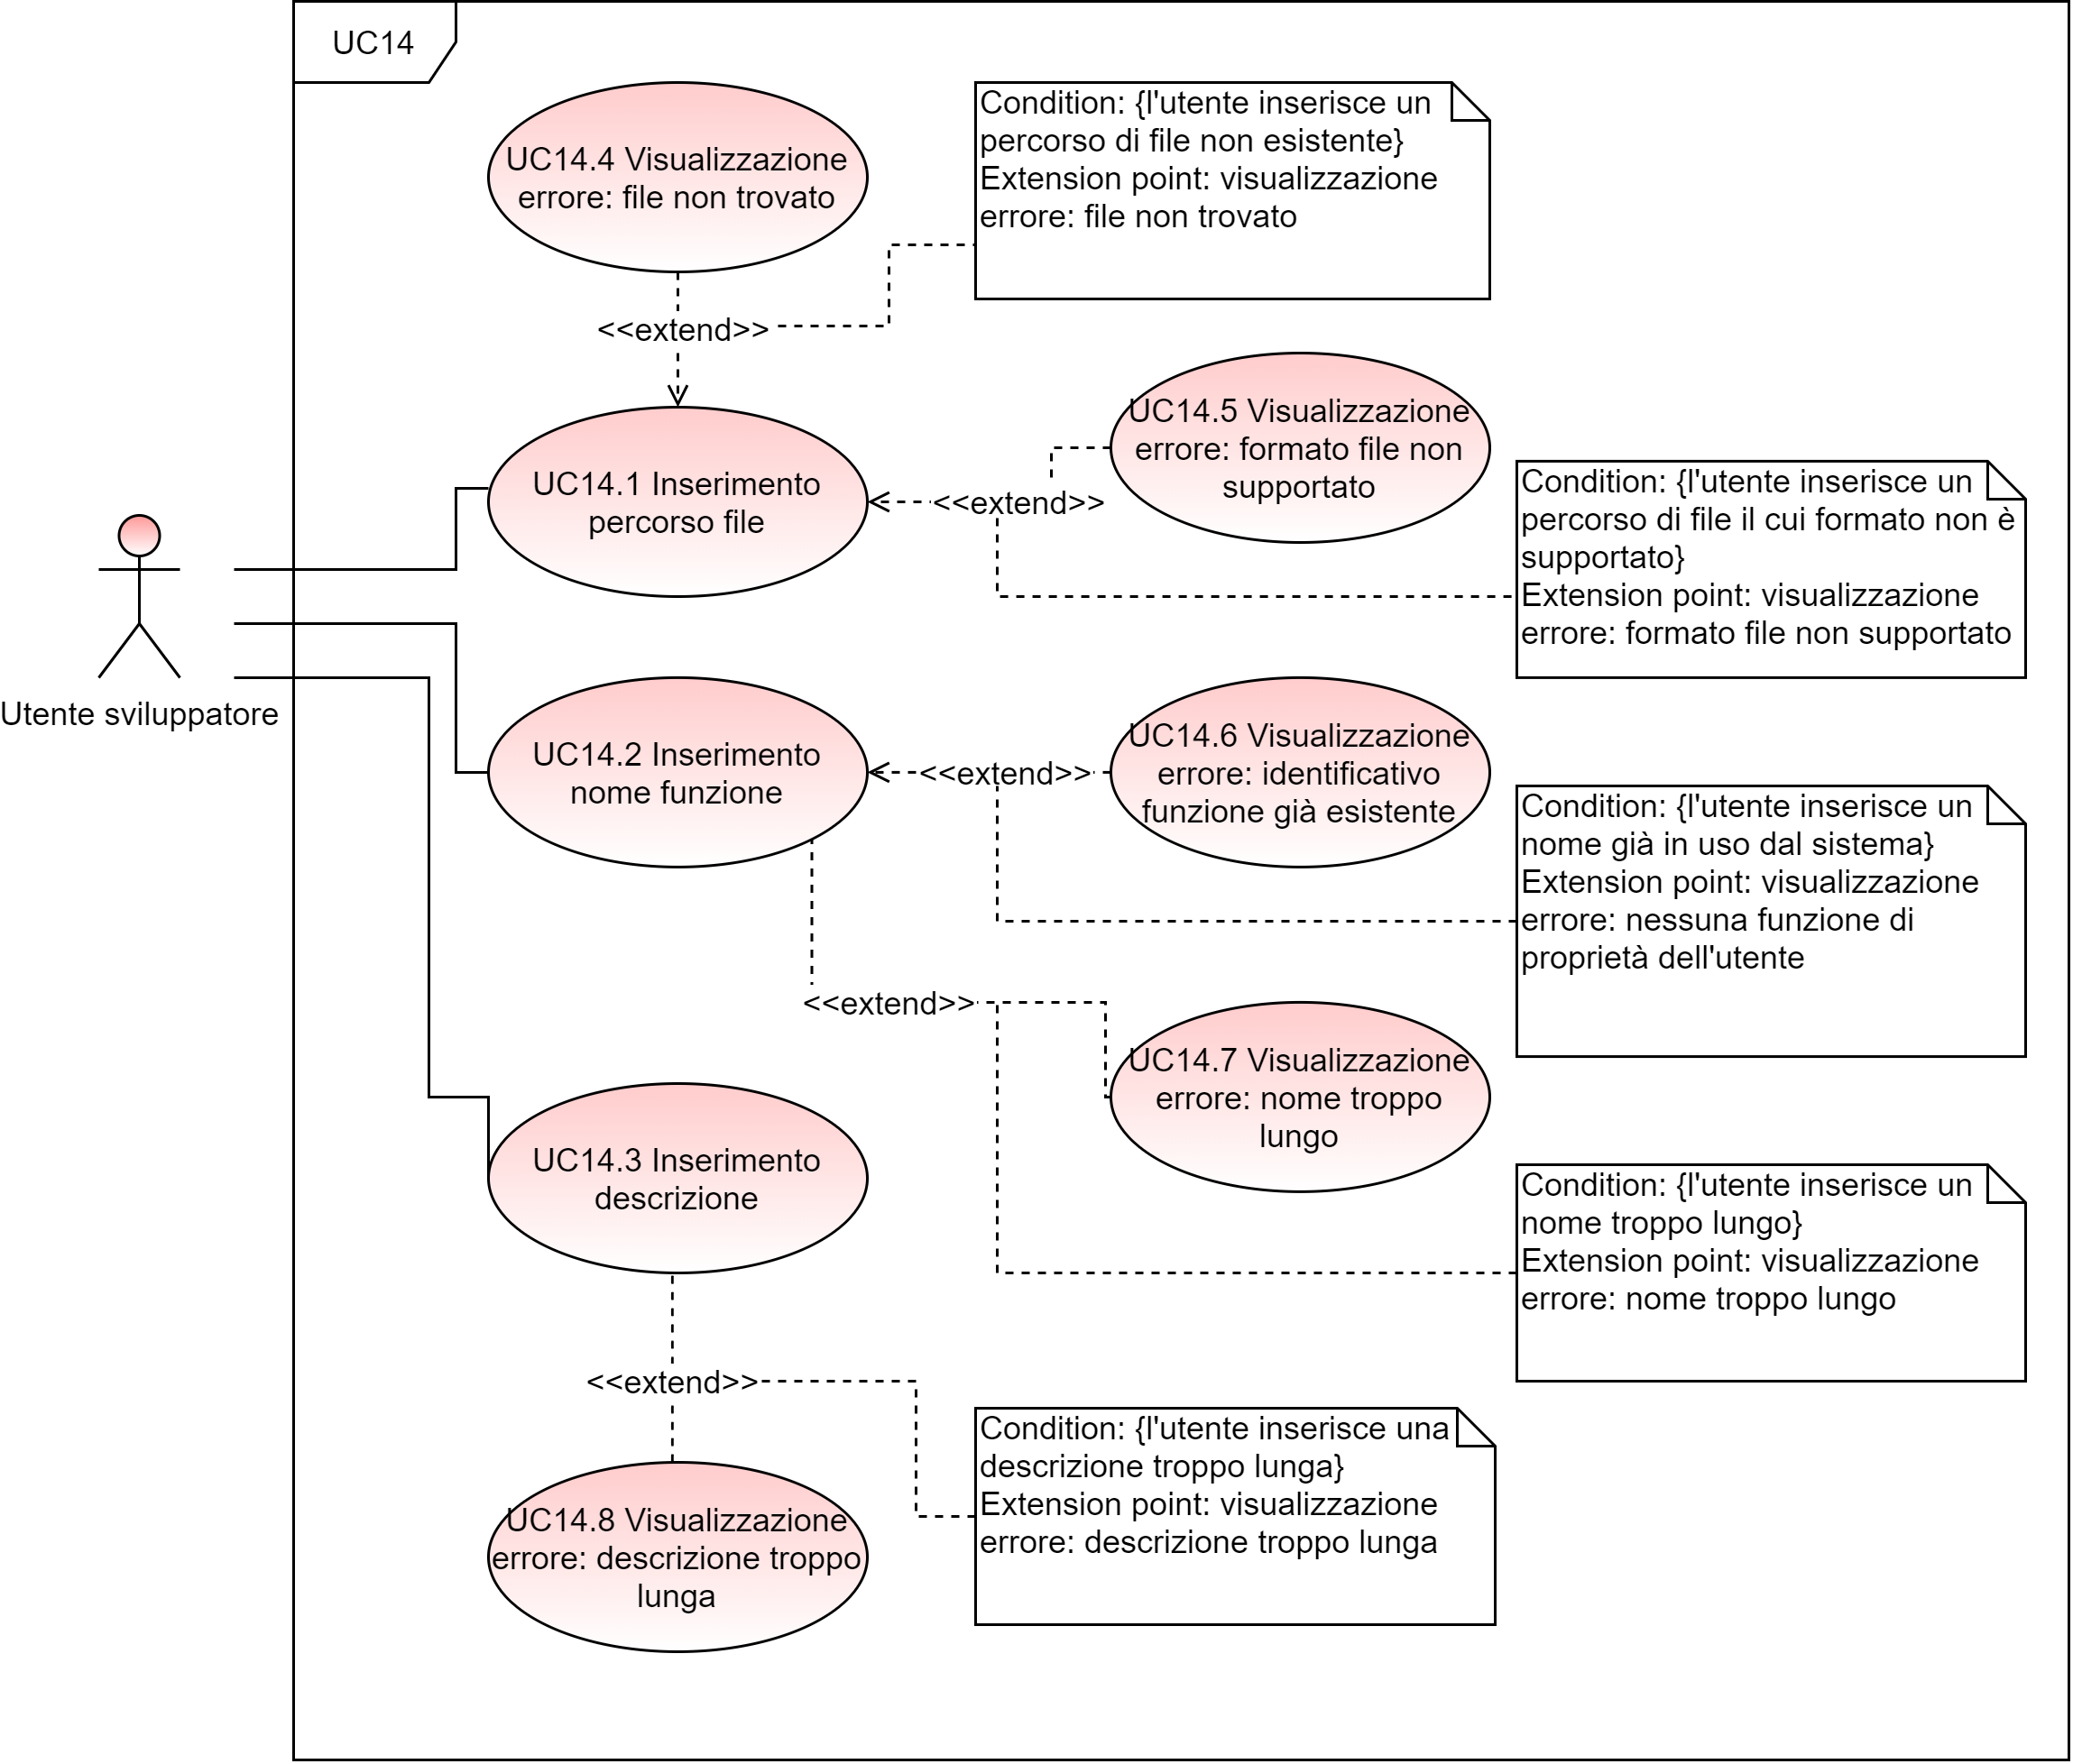
\includegraphics[scale=\ucs]{./res/img/UC14.png}
	\caption {UC14 - Deploy di funzione}
\end{figure}
\begin{itemize}
	\item \textbf{Attori primari:} \us{};
	\item \textbf{Attori secondari:} \re{};
	\item \textbf{Descrizione:} l’utente richiede di pubblicare una funzione eseguendo il comando \pdeploy{}. Il sistema pubblica la funzione; 
	\item \textbf{Scenario principale:} 
	\begin{itemize}
		\item l'utente inserisce correttamente ed esegue il comando \pdeploy{};
		\item la funzione viene pubblicata. 
	\end{itemize}
	\item \textbf{Estensioni:} 
	\begin{itemize}
		\item \textbf{UC19:} l’utente non dispone di credito sufficiente per pubblicare la funzione, di conseguenza viene visualizzato un messaggio di errore. 
	\end{itemize}
	\item \textbf{Precondizione:} l’utente ha avviato correttamente l’applicativo e desidera eseguire il deploy di una funzione; 
	\item \textbf{Postcondizione:} la nuova funzione inserita è disponibile presso il servizio. 
\end{itemize}
\subsubsection{UC14.1 - Inserimento percorso file}
\begin{itemize}
	\item \textbf{Attori primari:} \us{};
	\item \textbf{Descrizione:} al fine di portare a termine il processo di deploy l’utente inserisce il percorso del file contenente la funzione che si vuole pubblicare;  
	\item \textbf{Scenario principale:} l'utente inserisce il percorso del file contenente la funzione che si vuole pubblicare; 
	\item \textbf{Estensioni:} 
	\begin{itemize}
		\item \textbf{UC14.4:} l’utente inserisce un percorso di file non esistente. Viene di conseguenza visualizzato un messaggio di errore;
		\item \textbf{UC14.5:} l’utente inserisce un percorso di file il cui formato non è supportato dal sistema. Viene di conseguenza visualizzato un messaggio di errore. 
	\end{itemize}
	\item \textbf{Precondizione:} l’utente ha digitato il comando \deploy{}; 
	\item \textbf{Postcondizione:} il campo \textit{file\_path} contiene il percorso del file contenente la funzione che si vuole pubblicare. 
\end{itemize}
\subsubsection{UC14.2 - Inserimento nome funzione}
\begin{itemize}
	\item \textbf{Attori primari:} \us{};
	\item \textbf{Attori secondari:} \re{};
	\item \textbf{Descrizione:} al fine di portare a termine il processo di deploy l’utente inserisce il nome della funzione che si vuole pubblicare.  
	\item \textbf{Scenario principale:} l'utente inserisce il nome della funzione che vuole pubblicare;
	\item \textbf{Estensioni:} 
	\begin{itemize}
		\item \textbf{UC14.6:} l’utente inserisce un nome già in uso dal sistema. Viene di conseguenza visualizzato un messaggio di errore. 
		\item \textbf{UC14.7:} l’utente inserisce un nome troppo lungo. Viene di conseguenza visualizzato un messaggio di errore. 
	\end{itemize}
	\item \textbf{Precondizione:} L’utente ha digitato il comando deploy seguito dal campo \textit{file\_path};
	\item \textbf{Postcondizione:} il campo \textit{function\_name} contiene il nome della funzione che si vuole pubblicare.
\end{itemize}
\subsubsection{UC14.3 - Inserimento descrizione}
\begin{itemize}
	\item \textbf{Attori primari:} \us{};
	\item \textbf{Descrizione:} al fine di portare a termine il processo di deploy l’utente inserisce la descrizione della funzione che si vuole pubblicare;  
	\item \textbf{Scenario principale:} l’utente inserisce una descrizione della funzione che si vuole pubblicare;  
	\item \textbf{Estensioni:} 
	\begin{itemize}
		\item \textbf{UC14.8:} l’utente inserisce una descrizione troppo lunga. Viene di conseguenza visualizzato un messaggio di errore. 
	\end{itemize}
	\item \textbf{Precondizione:}  l’utente ha digitato il comando \deploy{} seguito dai campi \textit{file\_path} e \textit{function\_name};
	\item \textbf{Postcondizione:} il campo \textit{desc} contiene una descrizione della funzione che si vuole pubblicare.
\end{itemize}
\subsubsection{UC14.4 - Visualizzazione errore: file non trovato}
\begin{itemize}
	\item \textbf{Attori primari:} \us{};
	\item \textbf{Descrizione:} l’utente inserisce un percorso di file non esistente. Il sistema visualizza un messaggio di errore relativo alla mancata presenza del file;
	\item \textbf{Scenario principale:} viene visualizzato un messaggio di errore relativo alla mancata presenza del file;
	\item \textbf{Precondizione:} l’utente inserisce il percorso di un file non esistente; 
	\item \textbf{Postcondizione:} la CLI riporta un messaggio di errore.
\end{itemize}
\subsubsection{UC14.5 - Visualizzazione errore: formato non supportato}
\begin{itemize}
	\item \textbf{Attori primari:} \us{};
	\item \textbf{Descrizione:} l’utente inserisce un percorso di file di formato non supportato dal servizio. Il sistema visualizza un messaggio di errore relativo al formato errato.
	\item \textbf{Scenario principale:} viene visualizzato un messaggio di errore relativo al formato errato.
	\item \textbf{Precondizione:} l'utente inserisce un percorso di file di formato non supportato;
	\item \textbf{Postcondizione:} viene mostrato un messaggio di errore. 
\end{itemize}
\subsubsection{UC14.6 - Visualizzazione errore: nome funzione già esistente}
\begin{itemize}
	\item \textbf{Attori primari:} \us{};
	\item \textbf{Descrizione:} l’utente inserisce un nome di funzione già presente nel servizio. Il sistema visualizza un messaggio di errore relativo alla presenza del nome specificato;
	\item \textbf{Scenario principale:} viene visualizzato un messaggio di errore relativo alla presenza del nome specificato;
	\item \textbf{Precondizione:} il nome inserito dall’utente è già in uso all’interno del sistema; 
	\item \textbf{Postcondizione:} la CLI riporta un messaggio di errore.
\end{itemize}
\subsubsection{UC14.7 - Visualizzazione errore: nome troppo lungo}
\begin{itemize}
	\item \textbf{Attori primari:} \us{};
	\item \textbf{Descrizione:} l’utente inserisce un nome la cui lunghezza supera la lunghezza massima prevista. Il sistema visualizza un messaggio di errore specificando qual è la lunghezza massima consentita. 
	\item \textbf{Scenario principale:} viene visualizzato un messaggio di errore relativo all’eccessiva lunghezza del nome inserito;
	\item \textbf{Precondizione:} l'utente inserisce un nome troppo lungo;
	\item \textbf{Postcondizione:} l’utente visualizza un messaggio riguardante l’errore considerato. 
\end{itemize}
\subsubsection{UC14.8 - Visualizzazione errore: descrizione troppo lunga}
\begin{itemize}
	\item \textbf{Attori primari:} \us{};
	\item \textbf{Descrizione:} l’utente inserisce una descrizione la cui lunghezza supera la lunghezza massima prevista. Il sistema visualizza un messaggio di errore specificando qual è la lunghezza massima consentita;
	\item \textbf{Scenario principale:} viene visualizzato un messaggio di errore relativo all’eccessiva lunghezza della descrizione inserita; 
	\item \textbf{Precondizione:} l'utente inserisce una descrizione troppo lunga;
	\item \textbf{Postcondizione:} la CLI\ped{\textit{G}} riporta un messaggio di errore.
\end{itemize}

\subsubsection{UC15 - Modifica funzione }
\begin{figure}[H]
	\centering
	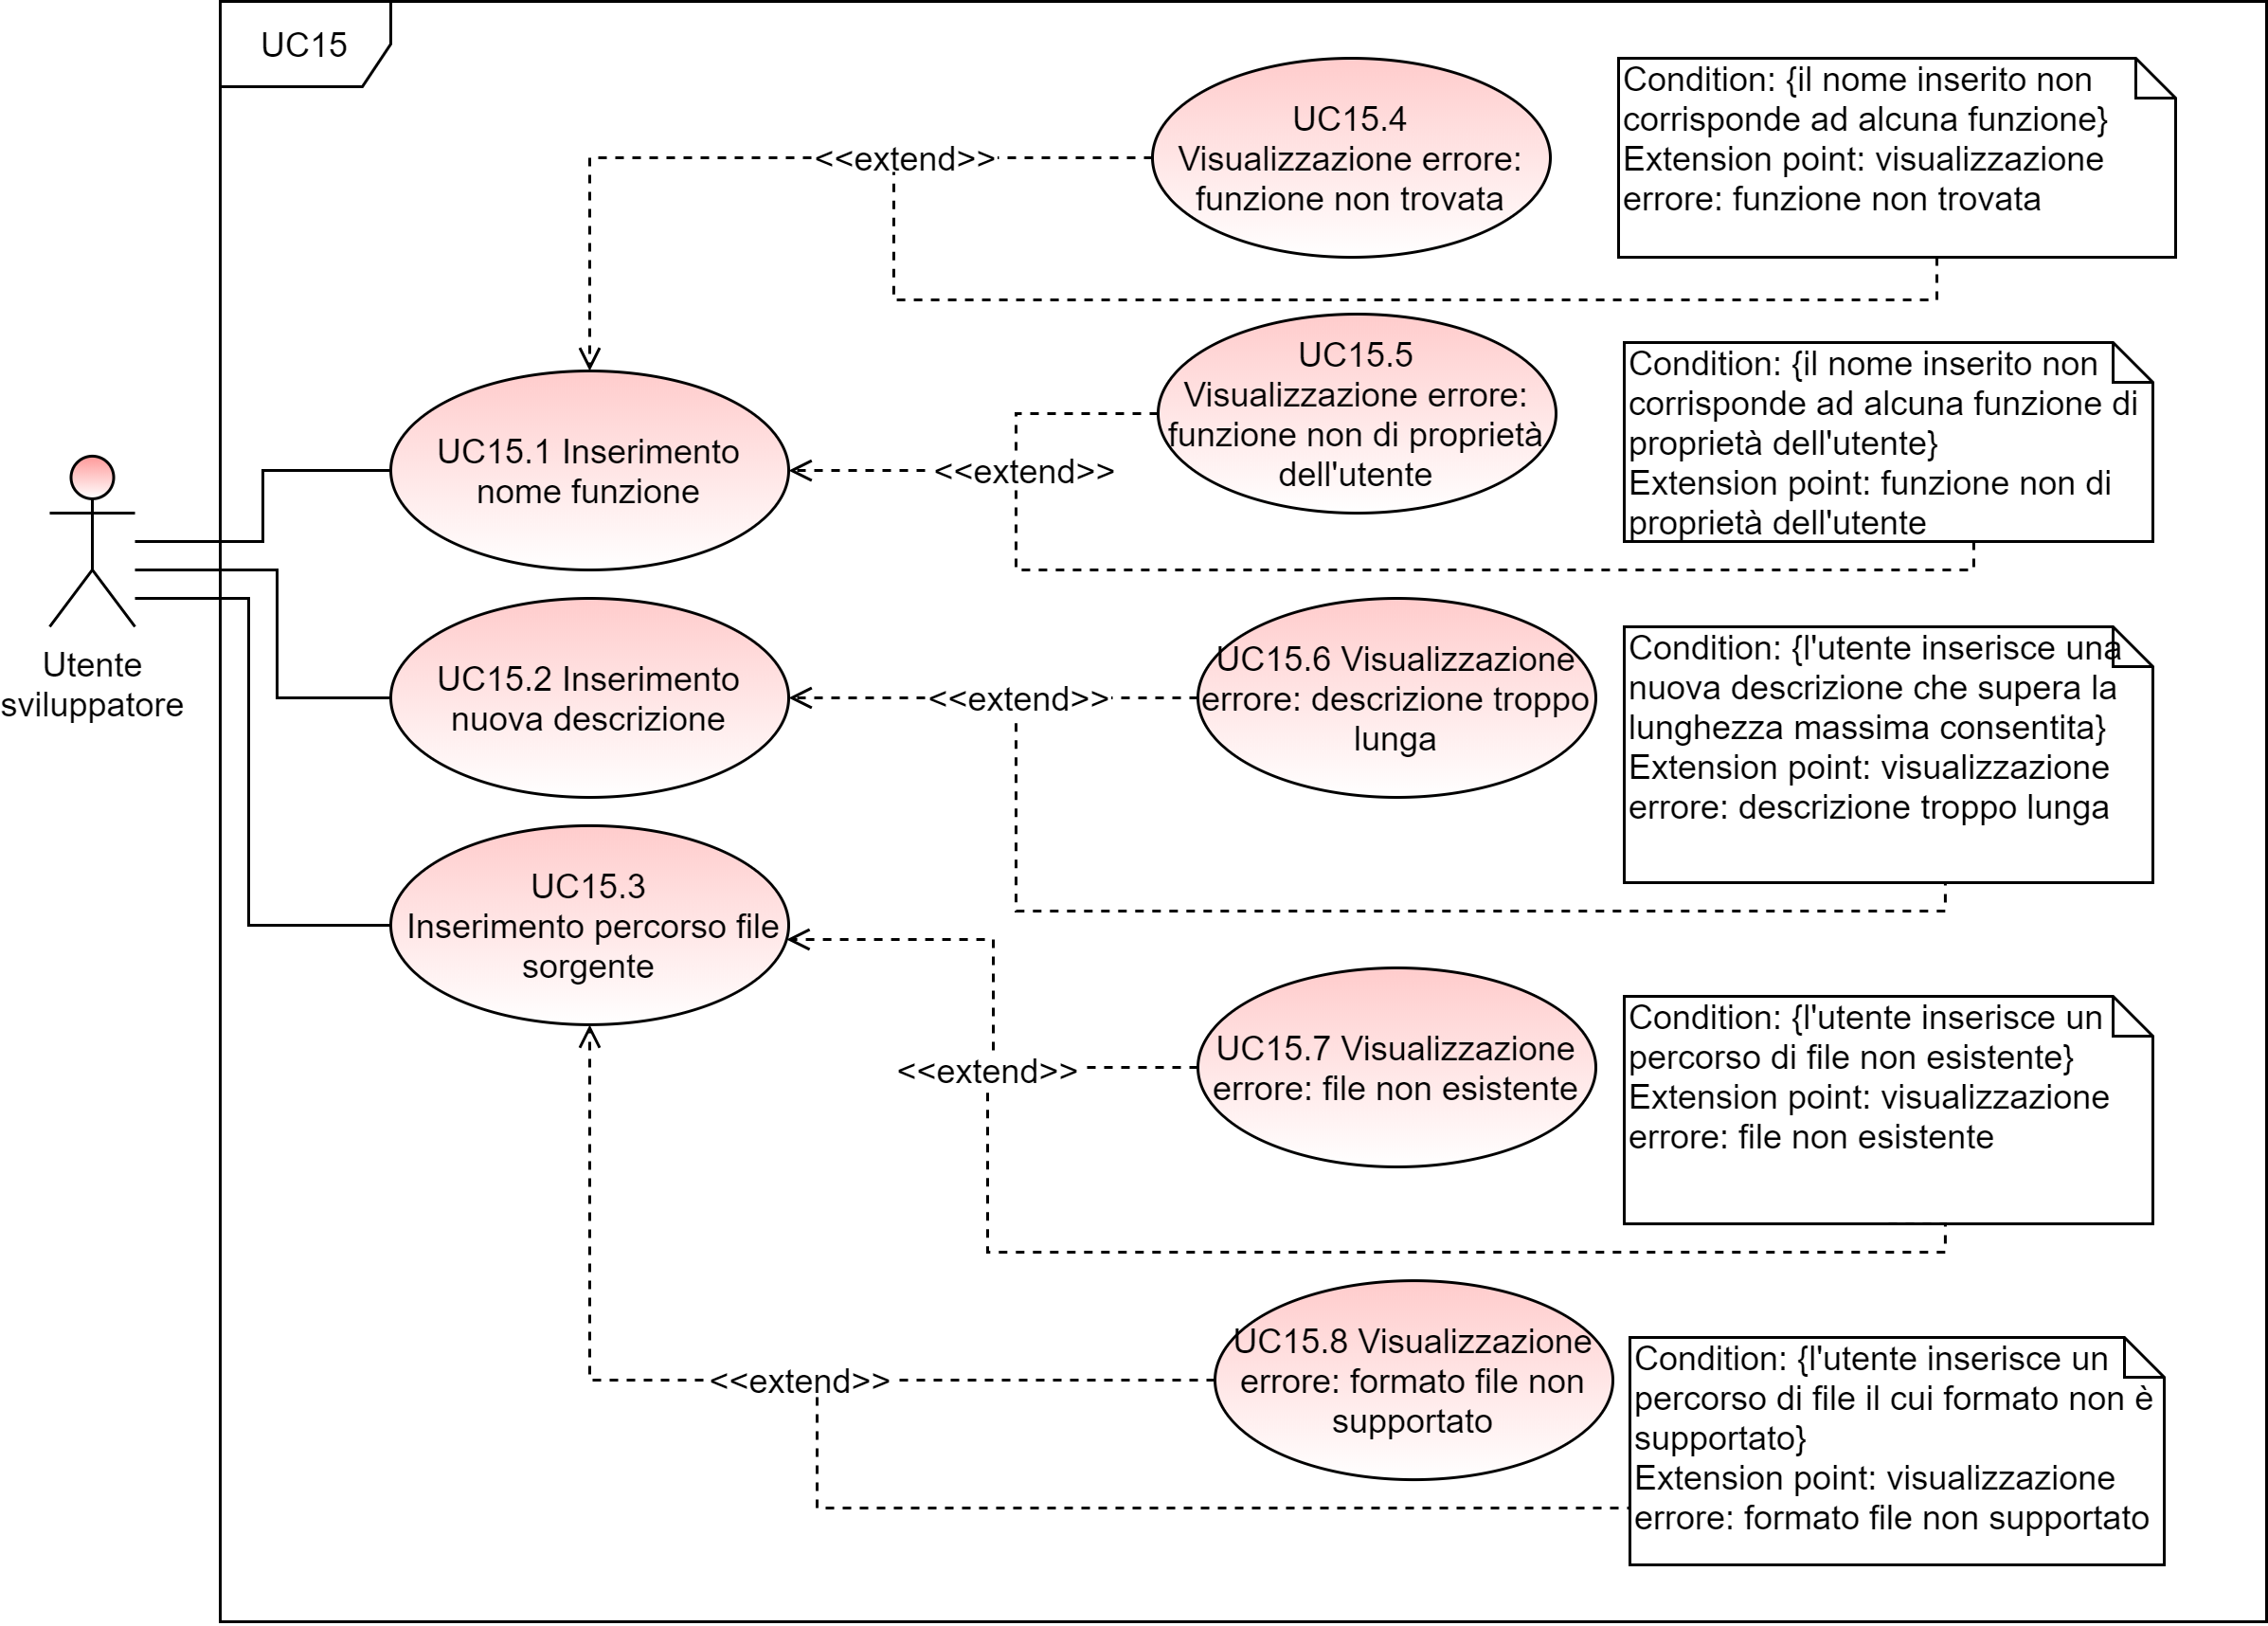
\includegraphics[scale=\ucs]{./res/img/UC15.png}
	\caption {UC15 - Modifica funzione }
\end{figure}
\begin{itemize}
	\item \textbf{Attori primari:} \us{};
	\item \textbf{Attori secondari:} \re{};
	\item \textbf{Descrizione:} l’utente richiede di modificare delle informazioni relative ad una sua funzione tramite il comando: \pedit{};
	\item \textbf{Scenario principale:} 
	\begin{itemize}
		\item l’utente richiede la modifica delle informazioni relative ad una sua funzione;
		\item il sistema apporta le modifiche richieste.  
	\end{itemize}
	\item \textbf{Precondizione:} l’utente ha eseguito il deploy\ped{\textit{G}} di almeno una funzione;
	\item \textbf{Postcondizione:} la funzione viene correttamente modificata. 
\end{itemize}
\subsubsection{UC15.1 - Inserimento valore da modificare}
\begin{figure}[h]
	\centering
	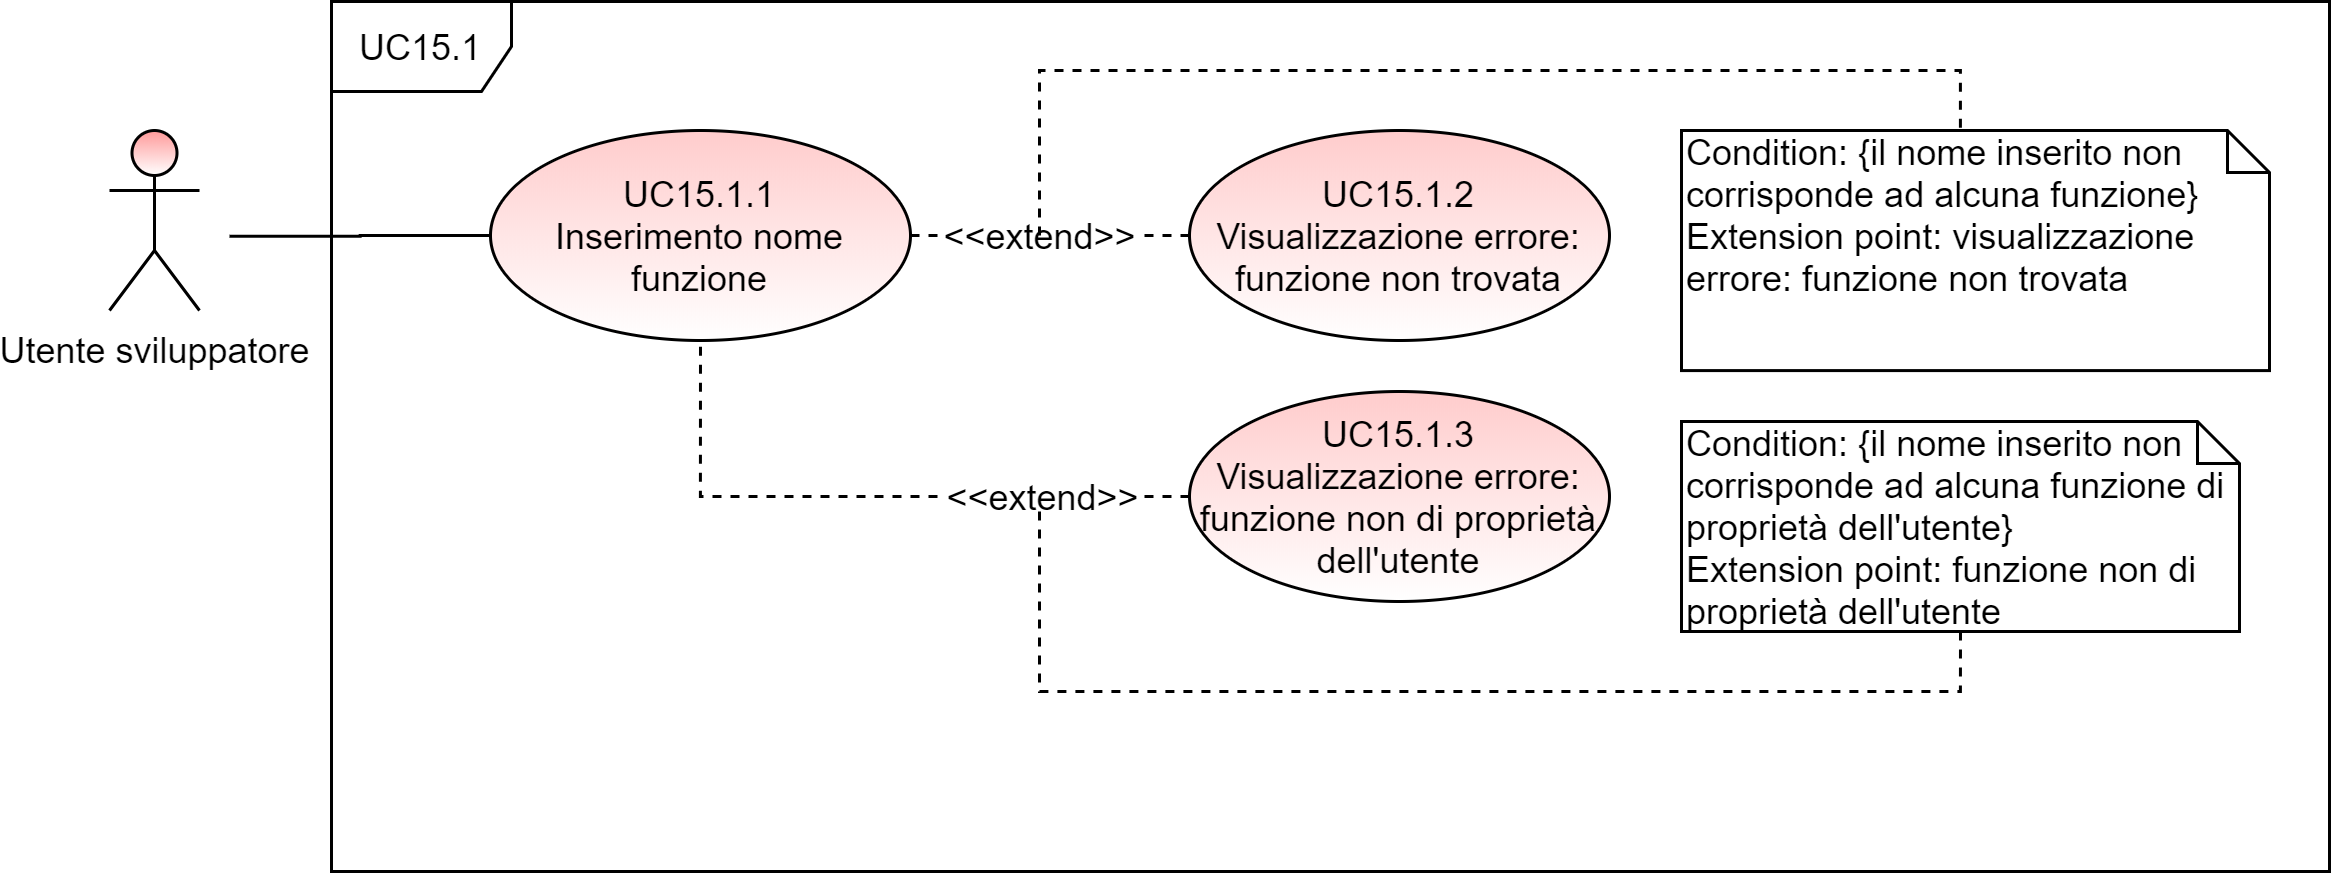
\includegraphics[scale=\ucs]{./res/img/UC15.1.png}
	\caption {UC15.1 - Inserimento valore da modificare}
\end{figure}
\begin{itemize}
	\item \textbf{Attori primari:} \us{};
	\item \textbf{Descrizione:} a seguito dell'inserimento del comando \edit{} l’utente procede con l’inserimento del nome della funzione considerata e delle modifiche da apportare; 
	\item \textbf{Scenario principale:} l'utente inserisce il comando \edit{} seguito dal nome della funzione e dalle infrormazioni da aggiornare. 
	\item \textbf{Specializzazioni:} 
	\begin{itemize}
		\item \textbf{UC15.2:} l’utente vuole modificare la descrizione della funzione considerata; 
		\item \textbf{UC15.3:} l’utente vuole modificare il codice della funzione. 
	\end{itemize}
	\item \textbf{Precondizione:} l’utente ha inserito all’interno della CLI il comando \edit{}; 
	\item \textbf{Postcondizione:} l’utente ha inserito correttamente le nuove informazioni relative alla funzione.
\end{itemize}
\subsubsection{UC15.2 - Inserimento nuova descrizione}
\begin{itemize}
	\item \textbf{Attori primari:} \us{};
	\item \textbf{Descrizione:} l'utente inserisce la nuova descrizione associata alla funzione che desidera modificare;
	\item \textbf{Scenario principale:} l’utente inserisce la nuova descrizione;  
	\item \textbf{Estensioni:} 
	\begin{itemize}
		\item \textbf{UC15.6:} se l’utente inserisce una nuova descrizione che supera la lunghezza massima consentita, viene visualizzato un apposito messaggio di errore. 
	\end{itemize}
	\item \textbf{Precondizione:} l’utente ha inserito all’interno della CLI\ped{\textit{G}} il comando \edit{} seguito dal flag \texttt{-d};
	\item \textbf{Postcondizione:} l’utente ha inserito correttamente la nuova descrizione.
\end{itemize}
\subsubsection{UC15.3 - Inserimento percorso file sorgente}
\begin{itemize}
	\item \textbf{Attori primari:} \us{};
	\item \textbf{Descrizione:} l'utente inserisce il comando \pedit{} \texttt{–c file\_path} indicando la volontà di voler modificare il codice associato alla funzione tramite il flag \texttt{-c}, e inserendo successivamente il percorso del file sorgente nel campo \texttt{file\_path}; 
	\item \textbf{Scenario principale:} l'utente inserisce il percorso del file contente il codice aggiornato dalla funzione. 
	\item \textbf{Estensioni:} 
	\begin{itemize}
		\item \textbf{UC15.5:} se l'utente inserisce il percorso di un file non presente viene visualizzato un apposito messaggio di errore.
		\item \textbf{UC15.6:} l’utente inserisce un percorso di file il cui formato non è supportato dal sistema. Viene di conseguenza visualizzato un messaggio di errore.
	\end{itemize}
	\item \textbf{Precondizione:} l’utente ha inserito all’interno della CLI\ped{\textit{G}} il comando \edit{}; 
	\item \textbf{Postcondizione:} l’utente ha inserito il percorso del file contenente il codice aggiornato della funzione.
\end{itemize}
\subsubsection{UC15.4 - Visualizzazione errore: funzione non trovata}
\begin{itemize}
	\item \textbf{Attori primari:} \us{};
	\item \textbf{Descrizione:} dopo aver inserito il nome di una funzione non presente all’interno della piattaforma \textit{Etherless}, l’utente visualizza un messaggio di errore; 
	\item \textbf{Scenario principale:} viene mostrato un messaggio di errore che informa l’utente dell’assenza della funzione precedentemente indicata;  
	\item \textbf{Precondizione:} il nome inserito dall’utente non corrisponde ad alcuna funzione;
	\item \textbf{Postcondizione:} la CLI\ped{\textit{G}} riporta un messaggio che descrive l’errore considerato. 
\end{itemize}
\subsubsection{UC15.5 - Visualizzazione errore: funzione non di proprietà dell’utente}
\begin{itemize}
	\item \textbf{Attori primari:} \us{};
	\item \textbf{Descrizione:} a seguito dell’inserimento di un nome relativo a una funzione non di proprietà dell’utente, viene visualizzato un errore;
	\item \textbf{Scenario principale:} viene visualizzato a schermo un messaggio di errore che informa l’utente che il nome inserito si riferisce ad una funzione non di sua proprietà;
	\item \textbf{Precondizione:} l’utente ha inserito il nome di una funzione non di sua proprietà; 
	\item \textbf{Postcondizione:} viene visualizzato un messaggio di errore. 
\end{itemize}
\subsubsection{UC15.6 - Visualizzazione errore: descrizione troppo lunga}
\begin{itemize}
	\item \textbf{Attori primari:} \us{};
	\item \textbf{Descrizione:} dopo aver inserito una descrizione di lunghezza maggiore rispetto a quella massima consentita l’utente visualizza un messaggio di errore; 
	\item \textbf{Scenario principale:} viene visualizzato un messaggio di errore che indica l’eccessiva lunghezza della descrizione inserita;  
	\item \textbf{Precondizione:} l’utente ha inserito la nuova descrizione della funzione;  
	\item \textbf{Postcondizione:} viene mostrato all’utente un messaggio che descrive l’errore considerato.  
\end{itemize}
\subsubsection{UC15.7 - Visualizzazione errore: file non esistente}
\begin{itemize}
	\item \textbf{Attori primari:} \us{};
	\item \textbf{Descrizione:} a seguito dell’inserimento del percorso di un file non esistente, viene visualizzato un messaggio di errore;  
	\item \textbf{Scenario principale:} viene mostrato un messaggio di errore che informa l’utente dell’assenza del file indicato; 
	\item \textbf{Precondizione:} l’utente ha inserito il percorso del file contenente il codice aggiornato della funzione considerata;  
	\item \textbf{Postcondizione:} la CLI\ped{\textit{G}} riporta un messaggio di errore. 
\end{itemize}
\subsubsection{UC15.8 - Visualizzazione errore: formato non supportato}
\begin{itemize}
	\item \textbf{Attori primari:} \us{};
	\item \textbf{Descrizione:} l’utente inserisce un percorso di file in un formato non supportato dal servizio. Il sistema visualizza un messaggio di errore relativo al formato errato;
	\item \textbf{Scenario principale:} viene visualizzato un messaggio di errore relativo al formato errato;
	\item \textbf{Precondizione:} l'utente inserisce un percorso di file in un formato non supportato;
	\item \textbf{Postcondizione:} viene mostrato un messaggio di errore. 
\end{itemize}


\subsubsection{UC16 - Cronologia di esecuzione}
\begin{figure}[H]
	\centering
	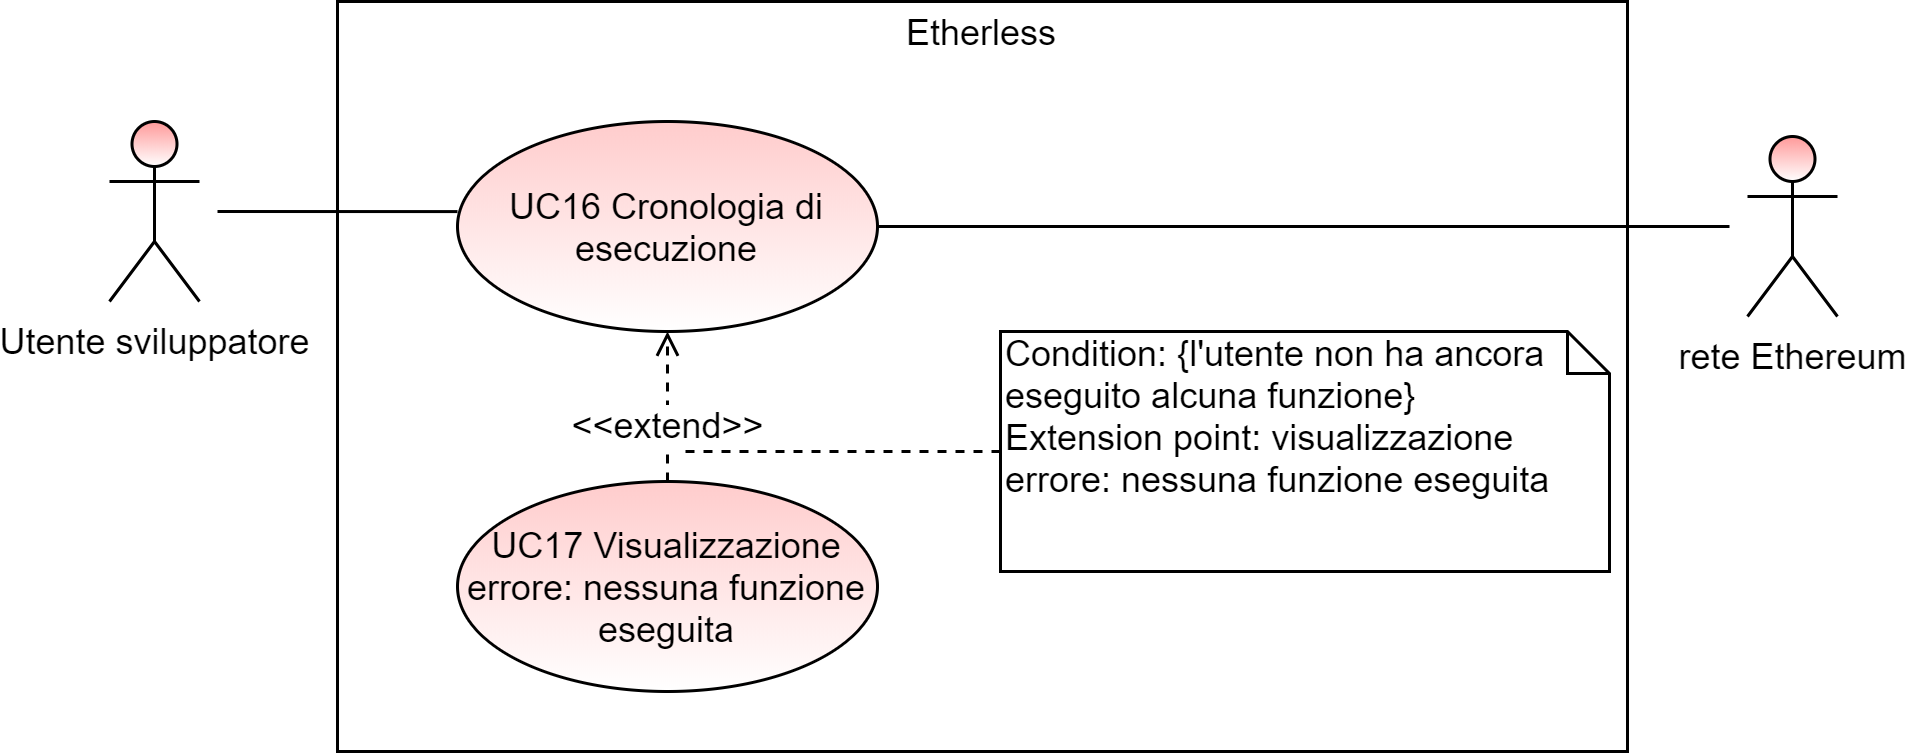
\includegraphics[scale=\ucs]{./res/img/UC16G.png}
	\caption {UC16 - Cronologia di esecuzione: schema generale}
\end{figure}
\begin{figure}[H]
	\centering
	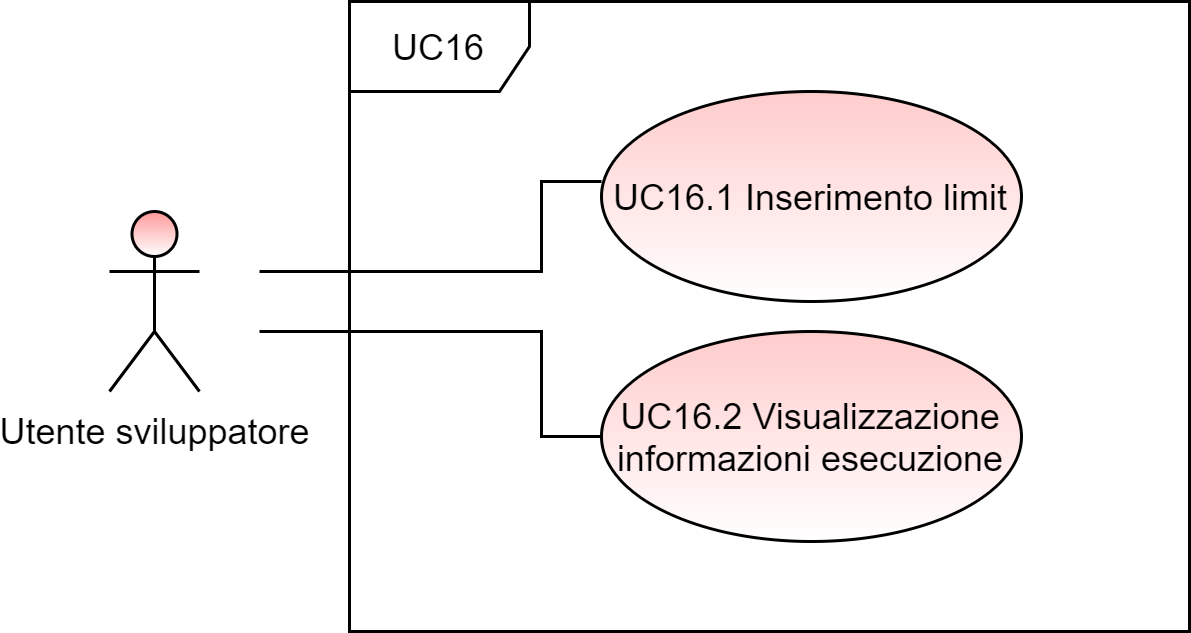
\includegraphics[scale=\ucs]{./res/img/UC16.png}
	\caption {UC16 - Cronologia di esecuzione}
\end{figure}
\begin{itemize}
	\item \textbf{Attori primari:} \us{};
	\item \textbf{Attori secondari:} \re{};
	\item \textbf{Descrizione:} l’utente ottiene le informazioni relative alla propria cronologia di invocazione di funzioni;
	\item \textbf{Scenario principale:} 
	\begin{itemize}
		\item l'utente inserisce il comando \history;  
		\item vengono visualizzate le informazioni relative alla cronologia delle chiamate dell’utente.
	\end{itemize}
	\item \textbf{Estensioni:} 
	\begin{itemize}
		\item \textbf{UC17:} nel caso l’utente non abbia mai eseguito alcuna funzione all’interno della piattaforma viene mostrato un apposito avviso.  
	\end{itemize}
	\item \textbf{Precondizione:} l’utente desidera visualizzare la propria cronologia di utilizzo della piattaforma \textit{Etherless}; 
	\item \textbf{Postcondizione:} viene visualizzata la cronologia di chiamate dell’utente.  
\end{itemize}
\subsubsection{UC16.1 - Inserimento limit}
\begin{itemize}
	\item \textbf{Attori primari:} \us{};
	\item \textbf{Descrizione:} l’utente può inserire un numero massimo di elementi da visualizzare tramite il flag \textit{-l}; 
	\item \textbf{Scenario principale:} l’utente inserisce il comando history seguito dal flag \textit{-l} e il relativo valore;
	\item \textbf{Precondizione:} l’utente ha inserito il comando “history” nella CLI;
	\item \textbf{Postcondizione:} è stato inserito correttamente il numero di massimo di risultati.
\end{itemize}
\subsubsection{UC16.2 - Visualizzazione informazioni esecuzione}
\begin{itemize}
	\item \textbf{Attori primari:} \us{};
	\item \textbf{Descrizione:} Per ogni elemento della cronologia di esecuzione vengono visualizzati:
	\begin{itemize}
		\item identificativo della richiesta; 
		\item nome della funzione richiamata; 
		\item eventuali parametri passati; 
		\item risultato dell’esecuzione; 
		\item data e orario della richiesta. 
	\end{itemize}
	\item \textbf{Scenario principale:} vengono visualizzate le informazioni rilevanti della singola esecuzione.
	\item \textbf{Precondizione:} l’utente ha inserito ed eseguito correttamente il comando \history{}; 
	\item \textbf{Postcondizione:} la CLI contiene le informazioni rilevanti della singola esecuzione;
\end{itemize}
\subsubsection{UC17 - Visualizzazione avviso: nessuna funzione eseguita}
\begin{itemize}
	\item \textbf{Attori primari:} \us{};
	\item \textbf{Descrizione:} l’utente dopo aver eseguito il comando history visualizza un avviso relativo alla mancanza di passate esecuzioni di funzioni all’interno della piattaforma \textit{Etherless};
	\item \textbf{Scenario principale:} 
	\begin{itemize}
		\item l’utente richiede la visualizzazione della propria cronologia di esecuzione tramite il comando \history{};
		\item viene visualizzato un avviso relativo alla mancanza di passate richieste di esecuzione.
	\end{itemize}
	\item \textbf{Precondizione:}  l’utente ha richiesto la visualizzazione della propria cronologia di esecuzione di funzioni non avendo prima eseguito alcuna funzione;
	\item \textbf{Postcondizione:} la CLI\ped{\textit{G}} riporta un avviso che descrive la situazione considerata.  
\end{itemize}
\subsubsection{UC18 - Rimozione funzione}
\begin{figure}[h]
	\centering
	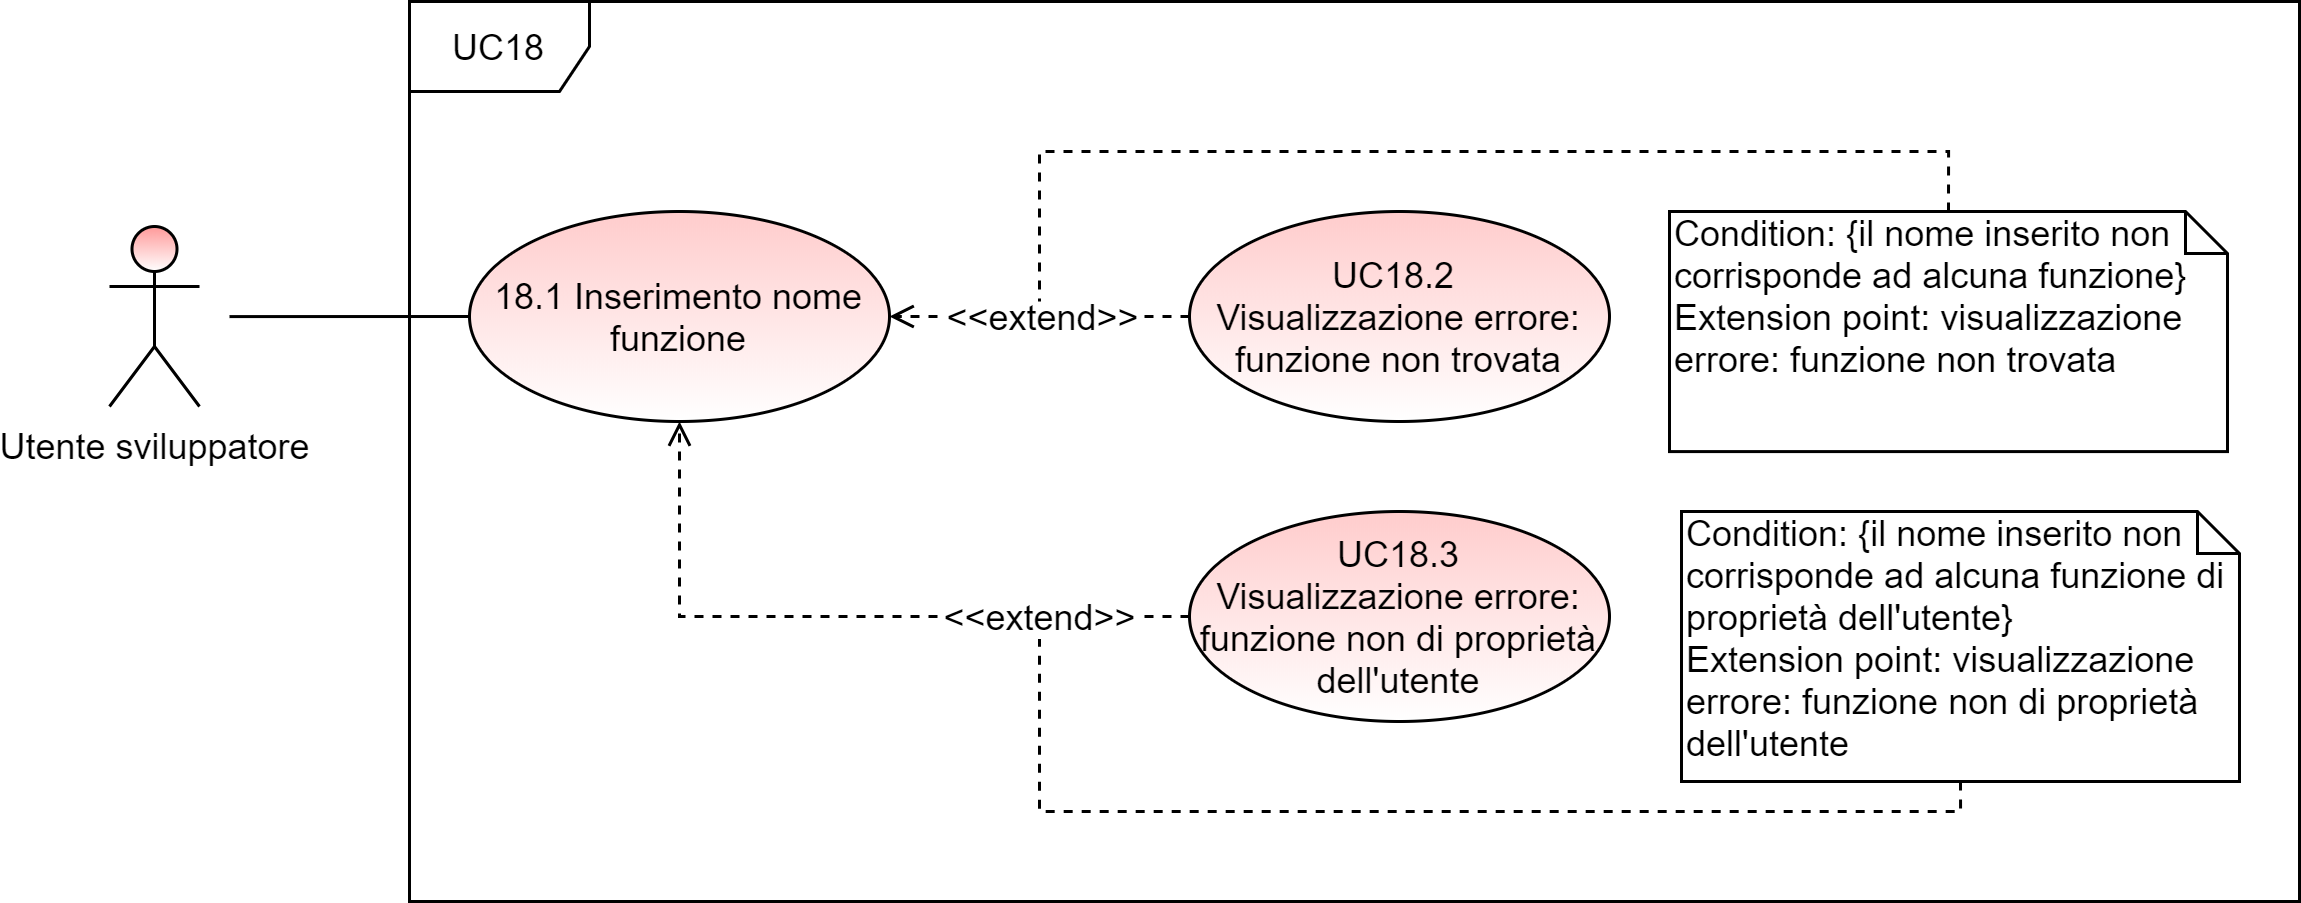
\includegraphics[scale=\ucs]{./res/img/UC18.png}
	\caption {UC18 - Rimozione funzione}
\end{figure}
\begin{itemize}
	\item \textbf{Attori primari:} \us{};
	\item \textbf{Attori secondari:} \re{};
	\item \textbf{Descrizione:} attraverso l’utilizzo del comando \delete{} l’utente può procedere alla rimozione di una funzione;  
	\item \textbf{Scenario principale:} 
	\begin{itemize}
		\item l’utente inserisce il comando \delete{} seguito dal nome della funzione da rimuovere; 
		\item la funzione viene rimossa con successo; 
	\end{itemize}
	\item \textbf{Precondizione:} l’utente vuole rimuovere una funzione dal sistema;  
	\item \textbf{Postcondizione:} la funzione è stata rimossa con successo dal sistema.
\end{itemize}
\subsubsection{UC18.1 - Inserimento nome funzione}
\begin{itemize}
	\item \textbf{Attori primari:} \us{};
	\item \textbf{Descrizione:} al fine di eseguire la procedura di rimozione di una funzione è richiesto l’inserimento del relativo nome; 
	\item \textbf{Scenario principale:} dopo aver deciso di eliminare una funzione l’utente inserisce nella CLI\ped{\textit{G}} il relativo nome; 
	\item \textbf{Estensioni:} 
	\begin{itemize}
		\item \textbf{UC18.2:} se l’utente inserisce un nome che non si riferisce ad alcuna funzione della piattaforma \textit{Etherless} viene mostrato un errore apposito;  
		\item \textbf{UC18.3:} se viene inserito un nome relativo ad una funzione non appartenente all’utente considerato, viene mostrato un relativo messaggio di errore. 
	\end{itemize}
	\item \textbf{Precondizione:} l’utente vuole rimuovere una determinata funzione dal sistema e ha già inserito il comando \delete{} nella CLI\ped{\textit{G}};  
	\item \textbf{Postcondizione:} l’utente ha inserito correttamente il nome della funzione che vuole rimuovere.  
\end{itemize}
\subsubsection{UC18.2 - Visualizzazione errore: funzione non trovata}
\begin{itemize}
	\item \textbf{Attori primari:} \us{};
	\item \textbf{Descrizione:} a seguito del tentativo di eliminazione di una funzione non presente all’interno del sistema, la CLI\ped{\textit{G}} visualizza un messaggio di errore;  
	\item \textbf{Scenario principale:} l’utente viene avvisato dell’assenza della funzione indicata tramite un messaggio di errore;
	\item \textbf{Precondizione:} l’utente ha inserito un nome che non si riferisce ad alcuna funzione presente all’interno del sistema;
	\item \textbf{Postcondizione:} la CLI\ped{\textit{G}} riporta un messaggio che descrive l’errore considerato.
\end{itemize}
\subsubsection{UC18.3 - Visualizzazione errore: funzione non di proprietà dell’utente}
\begin{itemize}
	\item \textbf{Attori primari:} \us{};
	\item \textbf{Descrizione:} l’utente tenta di eliminare una funzione che non è di sua proprietà; il sistema rileva tale situazione e mostra un messaggio di errore;
	\item \textbf{Scenario principale:} l’utente viene avvisato che la funzione non è di sua proprietà tramite la visualizzazione di un messaggio di errore;  
	\item \textbf{Precondizione:} l’utente ha inserito il nome di una funzione che non è di sua proprietà;  
	\item \textbf{Postcondizione:} viene mostrato un messaggio di errore.
\end{itemize}
\subsubsection{UC19 - Visualizzazione avviso: credito insufficiente}
\begin{figure}[h]
	\centering
	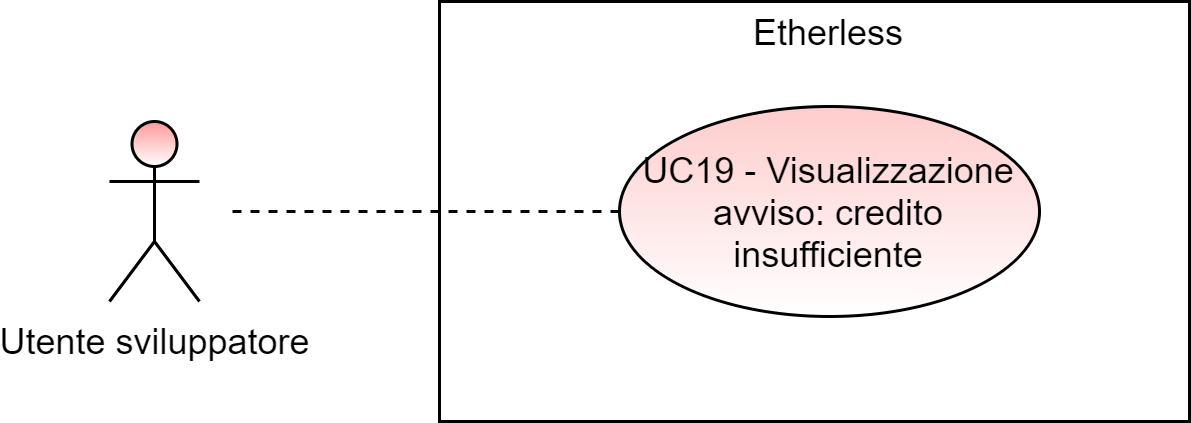
\includegraphics[scale=\ucs]{./res/img/UC19G.png}
	\caption {UC19 - Visualizzazione avviso: credito insufficiente - schema generale}
\end{figure}
\begin{itemize}
	\item \textbf{Attori primari:} \ua{};
	\item \textbf{Attori secondari:} \re{};
	\item \textbf{Descrizione:} l’utente richiede di eseguire un’operazione non avendo abbastanza credito a disposizione. Il sistema riporta un messaggio di errore relativo alla mancanza di credito; 
	\item \textbf{Scenario principale:} viene visualizzato un messaggio di errore relativo alla mancanza di credito necessario per portare a termine l’operazione;
	\item \textbf{Precondizione:} l’utente ha tentato di eseguire un’operazione a pagamento non avendo abbastanza credito a disposizione;  
	\item \textbf{Postcondizione:} la CLI riporta un messaggio di errore. 
\end{itemize}

\subsubsection{UC20 - Visualizzazione lista di tutte le funzioni}
\begin{figure}[H]
	\centering
	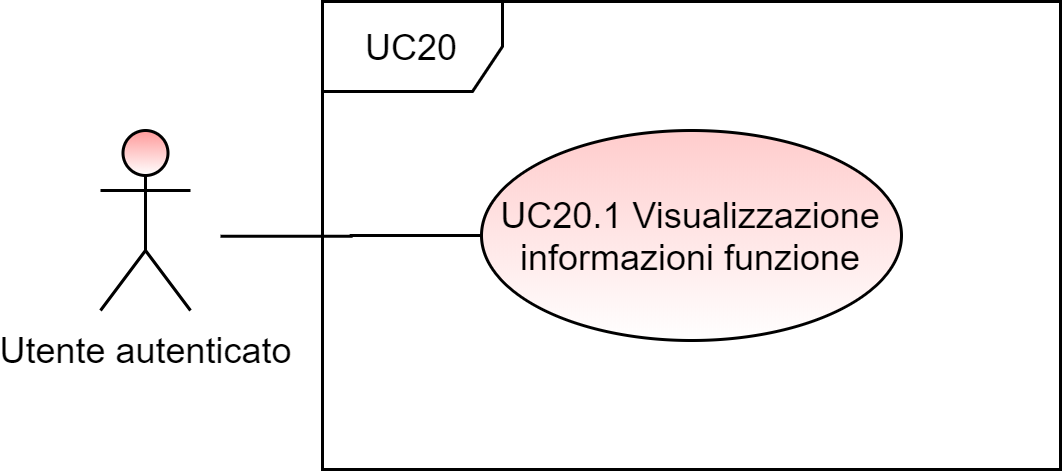
\includegraphics[scale=\ucs]{./res/img/UC20.png}
	\caption {UC20 -  Visualizzazione lista di tutte le funzioni}
\end{figure}
\begin{itemize}
	\item \textbf{Attori primari:} \ua{};
	\item \textbf{Descrizione:} l’utente richiede la visualizzazione della lista di tutte le funzioni fornite dal servizio eseguendo il comando \lista{}. Il sistema stampa a video tale lista; 
	\item \textbf{Scenario principale:} 
	\begin{itemize}
		\item l'utente inserisce correttamente ed esegue il comando \lista{}; 
		\item viene visualizzata la lista di tutte le funzioni disponibili presso il servizio.
	\end{itemize}
	\item \textbf{Estensioni:} 
	\begin{itemize}
		\item \textbf{UC22:} non è stata ancora pubblicata alcuna funzione, di conseguenza viene visualizzato un messaggio di avviso. 
	\end{itemize}
	\item \textbf{Precondizione:} l'utente inserisce correttamente ed esegue il comando \lista{};
	\item \textbf{Postcondizione:} la CLI\ped{\textit{G}} riporta la lista di tutte le funzioni fornite dal servizio.
\end{itemize}
\subsubsection{UC20.1 - Visualizzazione funzione }
\begin{itemize}
	\item \textbf{Attori primari:} \ua{};
	\item \textbf{Attori secondari:} \re{};
	\item \textbf{Descrizione:} vengono visualizzate le informazioni rilevanti della funzione, ovvero:
	\begin{itemize}
		\item firma della funzione;
		\item costo di esecuzione della funzione.
	\end{itemize}
	\item \textbf{Scenario principale:} vengono visualizzate le informazioni rilevanti della funzione;
	\item \textbf{Precondizione:} l'utente inserisce correttamente ed esegue il comando \lista{};
	\item \textbf{Postcondizione:} la CLI\ped{\textit{G}} riporta le informazioni rilevanti della funzione.  
\end{itemize}
\subsubsection{UC21 - Visualizzazione lista delle funzioni di proprietà dell’utente}
\begin{figure}[h]
	\centering
	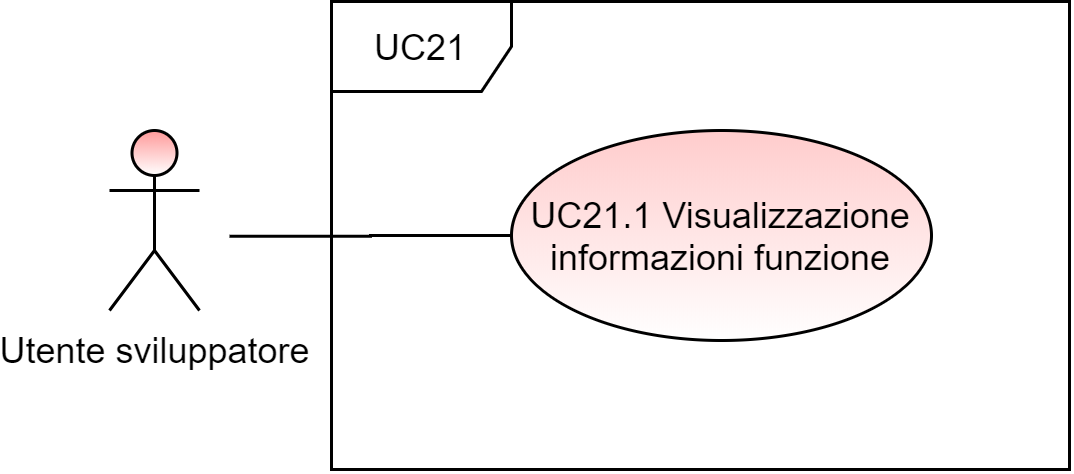
\includegraphics[scale=\ucs]{./res/img/UC21.png}
	\caption {UC21 - Visualizzazione lista funzioni di proprietà dell’utente}
\end{figure}
\begin{itemize}
	\item \textbf{Attori primari:} \us{};
	\item \textbf{Attori secondari:} \re{};
	\item \textbf{Descrizione:} l’utente richiede la visualizzazione della lista di tutte le funzioni di sua proprietà eseguendo il comando \plista{}. Il sistema stampa a video tale lista;
	\item \textbf{Scenario principale:} 
	\begin{itemize}
		\item l’utente inserisce correttamente ed esegue il comando \plista{};
		\item viene visualizzata la lista di tutte le funzioni di proprietà dell’utente. 
	\end{itemize}
	\item \textbf{Estensioni:} 
	\begin{itemize}
		\item \textbf{UC23:} l’utente non ha ancora pubblicato alcuna funzione, di conseguenza viene visualizzato un messaggio di avviso. 
	\end{itemize}
	\item \textbf{Precondizione:} l'utente inserisce correttamente ed esegue il comando \plista{};
	\item \textbf{Postcondizione:} la CLI\ped{\textit{G}} riporta la lista di tutte le funzioni di proprietà dell’utente. 
\end{itemize}
\subsubsection{UC21.1 - Visualizzazione funzione}
\begin{itemize}
	\item \textbf{Attori primari:} \us{};
	\item \textbf{Descrizione:} vengono visualizzate le informazioni rilevanti della funzione, ovvero:
	\begin{itemize}
		\item firma della funzione;
		\item costo di esecuzione della funzione;
		\item proprietario della funzione. 
	\end{itemize}
	\item \textbf{Scenario principale:} vengono visualizzate le informazioni rilevanti della funzione;
	\item \textbf{Precondizione:} l'utente inserisce correttamente ed esegue il comando \plista{};
	\item \textbf{Postcondizione:} la CLI\ped{\textit{G}} riporta le informazioni rilevanti della funzione.
\end{itemize}
\subsubsection{UC22 - Visualizzazione avviso: nessuna funzione pubblicata}
\begin{itemize}
	\item \textbf{Attori primari:} \ua{};
	\item \textbf{Attori secondari:} \re{};
	\item \textbf{Descrizione:} l’utente richiede la visualizzazione della lista di tutte le funzioni fornite dal servizio ma non viene trovata alcuna funzione. Il sistema visualizza un messaggio di avviso relativo alla mancata presenza di funzioni pubblicate; 
	\item \textbf{Scenario principale:} viene visualizzato un messaggio di avviso relativo all’assenza di funzioni pubblicate;
	\item \textbf{Precondizione:} nessun utente ha provveduto al caricamento di una propria funzione;
	\item \textbf{Postcondizione:}  l’utente visualizza un messaggio che spiega l’avviso considerato.
\end{itemize}
\subsubsection{UC23 - Visualizzazione avviso: nessuna funzione di proprietà dell’utente}
\begin{itemize}
	\item \textbf{Attori primari:} \us{};
	\item \textbf{Attori secondari:} \re{};
	\item \textbf{Descrizione:} l’utente richiede la visualizzazione della lista di tutte le funzioni di sua proprietà non avendo prima pubblicato alcuna funzione. Il sistema visualizza un messaggio di avviso relativo alla mancata presenza di funzioni di sua proprietà;
	\item \textbf{Scenario principale:} viene visualizzato un messaggio di avviso relativo alla mancata presenza di funzioni di proprietà dell’utente;
	\item \textbf{Precondizione:} l’utente corrente non ha funzioni di sua proprietà;
	\item \textbf{Postcondizione:} il sistema mostra un messaggio di avviso.
\end{itemize}

\subsubsection{UC24 - Visualizzazione informazioni funzione}
\begin{itemize}
	\item \textbf{Attori primari:} \ua{};
	\item \textbf{Descrizione:} vengono visualizzate le seguenti informazioni della funzione:
	\begin{itemize}
		\item firma della funzione;
		\item costo di esecuzione della funzione; 
		\item creatore della funzione; 
		\item descrizione completa della funzione.
	\end{itemize} 
	\item \textbf{Scenario principale:} vengono visualizzate le informazioni  dettagliate della funzione di interesse;
	\item \textbf{Estensioni: }
	\begin{itemize}
		\item \textbf{UC25}: nel caso in cui il nome inserito non identifichi alcuna funzione all'interno del sistema, viene visualizzato un messaggio di errore.
	\end{itemize}
	\item \textbf{Precondizione:} l’utente ha inserito ed eseguito correttamente il comando \pinfo{}; 
	\item \textbf{Postcondizione:} la CLI\ped{\textit{G}} riporta le informazioni dettagliate relative alla funzione. 
\end{itemize}

\subsubsection{UC25 - Visualizzazione errore: funzione non trovata}
\begin{itemize}
	\item \textbf{Attori primari:} \ua{};
	\item \textbf{Descrizione:} l’utente richiede la visualizzazione dei dettagli di una funzione specificando un identificativo non presente nel sistema. Il sistema riporta un messaggio di errore relativo alla mancata presenza della funzione; 
	\item \textbf{Scenario principale:} viene visualizzato un messaggio di errore relativo alla mancata presenza della funzione nel sistema; 
	\item \textbf{Precondizione:} l’utente esegue il comando info specificando l’identificativo di una funzione non esistente; 
	\item \textbf{Postcondizione:} la CLI\ped{\textit{G}} riporta un messaggio di errore.
\end{itemize}





